% Created by tikzDevice version 0.12.6 on 2025-04-17 10:37:42
% !TEX encoding = UTF-8 Unicode
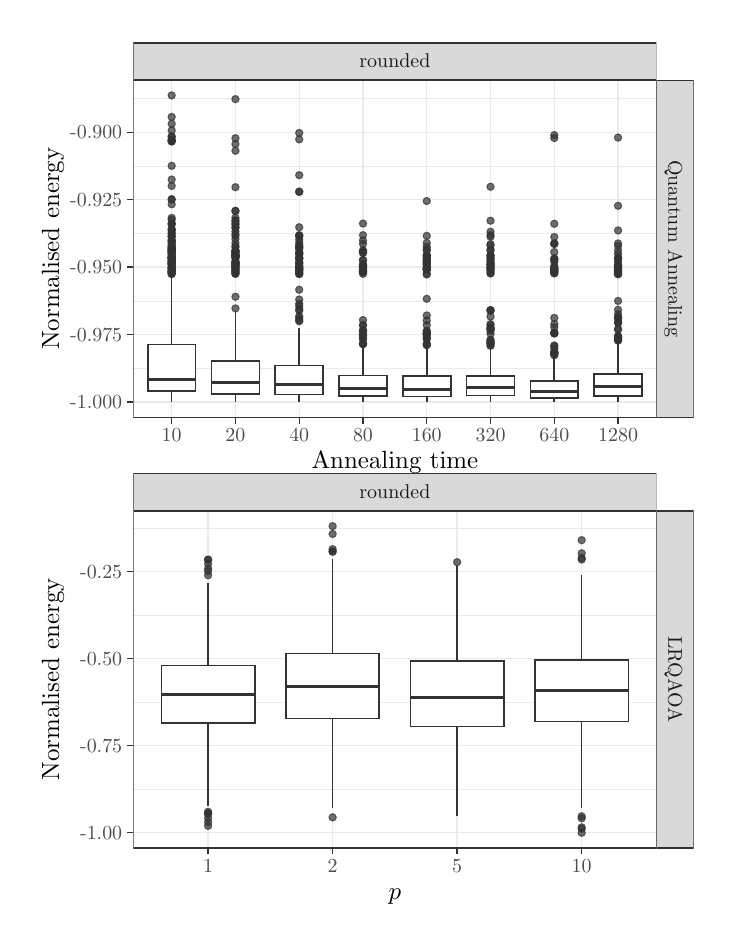
\begin{tikzpicture}[x=1pt,y=1pt]
\definecolor{fillColor}{RGB}{255,255,255}
\path[use as bounding box,fill=fillColor,fill opacity=0.00] (0,0) rectangle (251.81,322.31);
\begin{scope}
\path[clip] (  0.00,  0.00) rectangle (251.81,322.31);
\definecolor{drawColor}{RGB}{255,255,255}
\definecolor{fillColor}{RGB}{255,255,255}

\path[draw=drawColor,line width= 0.6pt,line join=round,line cap=round,fill=fillColor] (  0.00,  0.00) rectangle (251.81,322.31);
\end{scope}
\begin{scope}
\path[clip] (  5.50,161.16) rectangle (246.31,316.81);
\definecolor{drawColor}{RGB}{255,255,255}
\definecolor{fillColor}{RGB}{255,255,255}

\path[draw=drawColor,line width= 0.5pt,line join=round,line cap=round,fill=fillColor] (  5.50,161.16) rectangle (246.31,316.81);
\end{scope}
\begin{scope}
\path[clip] ( 38.20,181.51) rectangle (227.17,303.37);
\definecolor{fillColor}{RGB}{255,255,255}

\path[fill=fillColor] ( 38.20,181.51) rectangle (227.17,303.37);
\definecolor{drawColor}{gray}{0.92}

\path[draw=drawColor,line width= 0.2pt,line join=round] ( 38.20,199.23) --
	(227.17,199.23);

\path[draw=drawColor,line width= 0.2pt,line join=round] ( 38.20,223.58) --
	(227.17,223.58);

\path[draw=drawColor,line width= 0.2pt,line join=round] ( 38.20,247.94) --
	(227.17,247.94);

\path[draw=drawColor,line width= 0.2pt,line join=round] ( 38.20,272.29) --
	(227.17,272.29);

\path[draw=drawColor,line width= 0.2pt,line join=round] ( 38.20,296.65) --
	(227.17,296.65);

\path[draw=drawColor,line width= 0.5pt,line join=round] ( 38.20,187.05) --
	(227.17,187.05);

\path[draw=drawColor,line width= 0.5pt,line join=round] ( 38.20,211.40) --
	(227.17,211.40);

\path[draw=drawColor,line width= 0.5pt,line join=round] ( 38.20,235.76) --
	(227.17,235.76);

\path[draw=drawColor,line width= 0.5pt,line join=round] ( 38.20,260.12) --
	(227.17,260.12);

\path[draw=drawColor,line width= 0.5pt,line join=round] ( 38.20,284.47) --
	(227.17,284.47);

\path[draw=drawColor,line width= 0.5pt,line join=round] ( 52.03,181.51) --
	( 52.03,303.37);

\path[draw=drawColor,line width= 0.5pt,line join=round] ( 75.08,181.51) --
	( 75.08,303.37);

\path[draw=drawColor,line width= 0.5pt,line join=round] ( 98.12,181.51) --
	( 98.12,303.37);

\path[draw=drawColor,line width= 0.5pt,line join=round] (121.17,181.51) --
	(121.17,303.37);

\path[draw=drawColor,line width= 0.5pt,line join=round] (144.21,181.51) --
	(144.21,303.37);

\path[draw=drawColor,line width= 0.5pt,line join=round] (167.25,181.51) --
	(167.25,303.37);

\path[draw=drawColor,line width= 0.5pt,line join=round] (190.30,181.51) --
	(190.30,303.37);

\path[draw=drawColor,line width= 0.5pt,line join=round] (213.34,181.51) --
	(213.34,303.37);
\definecolor{drawColor}{RGB}{51,51,51}
\definecolor{fillColor}{RGB}{51,51,51}

\path[draw=drawColor,draw opacity=0.70,line width= 0.4pt,line join=round,line cap=round,fill=fillColor,fill opacity=0.70] ( 52.03,243.32) circle (  1.31);

\path[draw=drawColor,draw opacity=0.70,line width= 0.4pt,line join=round,line cap=round,fill=fillColor,fill opacity=0.70] ( 52.03,236.52) circle (  1.31);

\path[draw=drawColor,draw opacity=0.70,line width= 0.4pt,line join=round,line cap=round,fill=fillColor,fill opacity=0.70] ( 52.03,246.80) circle (  1.31);

\path[draw=drawColor,draw opacity=0.70,line width= 0.4pt,line join=round,line cap=round,fill=fillColor,fill opacity=0.70] ( 52.03,240.88) circle (  1.31);

\path[draw=drawColor,draw opacity=0.70,line width= 0.4pt,line join=round,line cap=round,fill=fillColor,fill opacity=0.70] ( 52.03,246.88) circle (  1.31);

\path[draw=drawColor,draw opacity=0.70,line width= 0.4pt,line join=round,line cap=round,fill=fillColor,fill opacity=0.70] ( 52.03,239.29) circle (  1.31);

\path[draw=drawColor,draw opacity=0.70,line width= 0.4pt,line join=round,line cap=round,fill=fillColor,fill opacity=0.70] ( 52.03,235.01) circle (  1.31);

\path[draw=drawColor,draw opacity=0.70,line width= 0.4pt,line join=round,line cap=round,fill=fillColor,fill opacity=0.70] ( 52.03,281.17) circle (  1.31);

\path[draw=drawColor,draw opacity=0.70,line width= 0.4pt,line join=round,line cap=round,fill=fillColor,fill opacity=0.70] ( 52.03,238.02) circle (  1.31);

\path[draw=drawColor,draw opacity=0.70,line width= 0.4pt,line join=round,line cap=round,fill=fillColor,fill opacity=0.70] ( 52.03,238.91) circle (  1.31);

\path[draw=drawColor,draw opacity=0.70,line width= 0.4pt,line join=round,line cap=round,fill=fillColor,fill opacity=0.70] ( 52.03,239.13) circle (  1.31);

\path[draw=drawColor,draw opacity=0.70,line width= 0.4pt,line join=round,line cap=round,fill=fillColor,fill opacity=0.70] ( 52.03,242.83) circle (  1.31);

\path[draw=drawColor,draw opacity=0.70,line width= 0.4pt,line join=round,line cap=round,fill=fillColor,fill opacity=0.70] ( 52.03,249.62) circle (  1.31);

\path[draw=drawColor,draw opacity=0.70,line width= 0.4pt,line join=round,line cap=round,fill=fillColor,fill opacity=0.70] ( 52.03,235.60) circle (  1.31);

\path[draw=drawColor,draw opacity=0.70,line width= 0.4pt,line join=round,line cap=round,fill=fillColor,fill opacity=0.70] ( 52.03,272.38) circle (  1.31);

\path[draw=drawColor,draw opacity=0.70,line width= 0.4pt,line join=round,line cap=round,fill=fillColor,fill opacity=0.70] ( 52.03,233.90) circle (  1.31);

\path[draw=drawColor,draw opacity=0.70,line width= 0.4pt,line join=round,line cap=round,fill=fillColor,fill opacity=0.70] ( 52.03,252.89) circle (  1.31);

\path[draw=drawColor,draw opacity=0.70,line width= 0.4pt,line join=round,line cap=round,fill=fillColor,fill opacity=0.70] ( 52.03,238.96) circle (  1.31);

\path[draw=drawColor,draw opacity=0.70,line width= 0.4pt,line join=round,line cap=round,fill=fillColor,fill opacity=0.70] ( 52.03,242.23) circle (  1.31);

\path[draw=drawColor,draw opacity=0.70,line width= 0.4pt,line join=round,line cap=round,fill=fillColor,fill opacity=0.70] ( 52.03,239.09) circle (  1.31);

\path[draw=drawColor,draw opacity=0.70,line width= 0.4pt,line join=round,line cap=round,fill=fillColor,fill opacity=0.70] ( 52.03,235.57) circle (  1.31);

\path[draw=drawColor,draw opacity=0.70,line width= 0.4pt,line join=round,line cap=round,fill=fillColor,fill opacity=0.70] ( 52.03,233.61) circle (  1.31);

\path[draw=drawColor,draw opacity=0.70,line width= 0.4pt,line join=round,line cap=round,fill=fillColor,fill opacity=0.70] ( 52.03,242.39) circle (  1.31);

\path[draw=drawColor,draw opacity=0.70,line width= 0.4pt,line join=round,line cap=round,fill=fillColor,fill opacity=0.70] ( 52.03,242.60) circle (  1.31);

\path[draw=drawColor,draw opacity=0.70,line width= 0.4pt,line join=round,line cap=round,fill=fillColor,fill opacity=0.70] ( 52.03,233.28) circle (  1.31);

\path[draw=drawColor,draw opacity=0.70,line width= 0.4pt,line join=round,line cap=round,fill=fillColor,fill opacity=0.70] ( 52.03,239.23) circle (  1.31);

\path[draw=drawColor,draw opacity=0.70,line width= 0.4pt,line join=round,line cap=round,fill=fillColor,fill opacity=0.70] ( 52.03,238.36) circle (  1.31);

\path[draw=drawColor,draw opacity=0.70,line width= 0.4pt,line join=round,line cap=round,fill=fillColor,fill opacity=0.70] ( 52.03,245.09) circle (  1.31);

\path[draw=drawColor,draw opacity=0.70,line width= 0.4pt,line join=round,line cap=round,fill=fillColor,fill opacity=0.70] ( 52.03,253.57) circle (  1.31);

\path[draw=drawColor,draw opacity=0.70,line width= 0.4pt,line join=round,line cap=round,fill=fillColor,fill opacity=0.70] ( 52.03,243.31) circle (  1.31);

\path[draw=drawColor,draw opacity=0.70,line width= 0.4pt,line join=round,line cap=round,fill=fillColor,fill opacity=0.70] ( 52.03,242.07) circle (  1.31);

\path[draw=drawColor,draw opacity=0.70,line width= 0.4pt,line join=round,line cap=round,fill=fillColor,fill opacity=0.70] ( 52.03,234.24) circle (  1.31);

\path[draw=drawColor,draw opacity=0.70,line width= 0.4pt,line join=round,line cap=round,fill=fillColor,fill opacity=0.70] ( 52.03,239.64) circle (  1.31);

\path[draw=drawColor,draw opacity=0.70,line width= 0.4pt,line join=round,line cap=round,fill=fillColor,fill opacity=0.70] ( 52.03,238.96) circle (  1.31);

\path[draw=drawColor,draw opacity=0.70,line width= 0.4pt,line join=round,line cap=round,fill=fillColor,fill opacity=0.70] ( 52.03,260.33) circle (  1.31);

\path[draw=drawColor,draw opacity=0.70,line width= 0.4pt,line join=round,line cap=round,fill=fillColor,fill opacity=0.70] ( 52.03,237.37) circle (  1.31);

\path[draw=drawColor,draw opacity=0.70,line width= 0.4pt,line join=round,line cap=round,fill=fillColor,fill opacity=0.70] ( 52.03,290.06) circle (  1.31);

\path[draw=drawColor,draw opacity=0.70,line width= 0.4pt,line join=round,line cap=round,fill=fillColor,fill opacity=0.70] ( 52.03,235.60) circle (  1.31);

\path[draw=drawColor,draw opacity=0.70,line width= 0.4pt,line join=round,line cap=round,fill=fillColor,fill opacity=0.70] ( 52.03,281.62) circle (  1.31);

\path[draw=drawColor,draw opacity=0.70,line width= 0.4pt,line join=round,line cap=round,fill=fillColor,fill opacity=0.70] ( 52.03,241.08) circle (  1.31);

\path[draw=drawColor,draw opacity=0.70,line width= 0.4pt,line join=round,line cap=round,fill=fillColor,fill opacity=0.70] ( 52.03,234.35) circle (  1.31);

\path[draw=drawColor,draw opacity=0.70,line width= 0.4pt,line join=round,line cap=round,fill=fillColor,fill opacity=0.70] ( 52.03,241.95) circle (  1.31);

\path[draw=drawColor,draw opacity=0.70,line width= 0.4pt,line join=round,line cap=round,fill=fillColor,fill opacity=0.70] ( 52.03,235.29) circle (  1.31);

\path[draw=drawColor,draw opacity=0.70,line width= 0.4pt,line join=round,line cap=round,fill=fillColor,fill opacity=0.70] ( 52.03,236.94) circle (  1.31);

\path[draw=drawColor,draw opacity=0.70,line width= 0.4pt,line join=round,line cap=round,fill=fillColor,fill opacity=0.70] ( 52.03,283.05) circle (  1.31);

\path[draw=drawColor,draw opacity=0.70,line width= 0.4pt,line join=round,line cap=round,fill=fillColor,fill opacity=0.70] ( 52.03,251.28) circle (  1.31);

\path[draw=drawColor,draw opacity=0.70,line width= 0.4pt,line join=round,line cap=round,fill=fillColor,fill opacity=0.70] ( 52.03,281.72) circle (  1.31);

\path[draw=drawColor,draw opacity=0.70,line width= 0.4pt,line join=round,line cap=round,fill=fillColor,fill opacity=0.70] ( 52.03,241.12) circle (  1.31);

\path[draw=drawColor,draw opacity=0.70,line width= 0.4pt,line join=round,line cap=round,fill=fillColor,fill opacity=0.70] ( 52.03,234.84) circle (  1.31);

\path[draw=drawColor,draw opacity=0.70,line width= 0.4pt,line join=round,line cap=round,fill=fillColor,fill opacity=0.70] ( 52.03,282.82) circle (  1.31);

\path[draw=drawColor,draw opacity=0.70,line width= 0.4pt,line join=round,line cap=round,fill=fillColor,fill opacity=0.70] ( 52.03,237.79) circle (  1.31);

\path[draw=drawColor,draw opacity=0.70,line width= 0.4pt,line join=round,line cap=round,fill=fillColor,fill opacity=0.70] ( 52.03,258.48) circle (  1.31);

\path[draw=drawColor,draw opacity=0.70,line width= 0.4pt,line join=round,line cap=round,fill=fillColor,fill opacity=0.70] ( 52.03,243.21) circle (  1.31);

\path[draw=drawColor,draw opacity=0.70,line width= 0.4pt,line join=round,line cap=round,fill=fillColor,fill opacity=0.70] ( 52.03,260.16) circle (  1.31);

\path[draw=drawColor,draw opacity=0.70,line width= 0.4pt,line join=round,line cap=round,fill=fillColor,fill opacity=0.70] ( 52.03,236.90) circle (  1.31);

\path[draw=drawColor,draw opacity=0.70,line width= 0.4pt,line join=round,line cap=round,fill=fillColor,fill opacity=0.70] ( 52.03,240.36) circle (  1.31);

\path[draw=drawColor,draw opacity=0.70,line width= 0.4pt,line join=round,line cap=round,fill=fillColor,fill opacity=0.70] ( 52.03,234.49) circle (  1.31);

\path[draw=drawColor,draw opacity=0.70,line width= 0.4pt,line join=round,line cap=round,fill=fillColor,fill opacity=0.70] ( 52.03,248.00) circle (  1.31);

\path[draw=drawColor,draw opacity=0.70,line width= 0.4pt,line join=round,line cap=round,fill=fillColor,fill opacity=0.70] ( 52.03,244.98) circle (  1.31);

\path[draw=drawColor,draw opacity=0.70,line width= 0.4pt,line join=round,line cap=round,fill=fillColor,fill opacity=0.70] ( 52.03,233.77) circle (  1.31);

\path[draw=drawColor,draw opacity=0.70,line width= 0.4pt,line join=round,line cap=round,fill=fillColor,fill opacity=0.70] ( 52.03,281.24) circle (  1.31);

\path[draw=drawColor,draw opacity=0.70,line width= 0.4pt,line join=round,line cap=round,fill=fillColor,fill opacity=0.70] ( 52.03,297.83) circle (  1.31);

\path[draw=drawColor,draw opacity=0.70,line width= 0.4pt,line join=round,line cap=round,fill=fillColor,fill opacity=0.70] ( 52.03,267.43) circle (  1.31);

\path[draw=drawColor,draw opacity=0.70,line width= 0.4pt,line join=round,line cap=round,fill=fillColor,fill opacity=0.70] ( 52.03,285.19) circle (  1.31);

\path[draw=drawColor,draw opacity=0.70,line width= 0.4pt,line join=round,line cap=round,fill=fillColor,fill opacity=0.70] ( 52.03,281.66) circle (  1.31);

\path[draw=drawColor,draw opacity=0.70,line width= 0.4pt,line join=round,line cap=round,fill=fillColor,fill opacity=0.70] ( 52.03,234.10) circle (  1.31);

\path[draw=drawColor,draw opacity=0.70,line width= 0.4pt,line join=round,line cap=round,fill=fillColor,fill opacity=0.70] ( 52.03,246.95) circle (  1.31);

\path[draw=drawColor,draw opacity=0.70,line width= 0.4pt,line join=round,line cap=round,fill=fillColor,fill opacity=0.70] ( 52.03,241.09) circle (  1.31);

\path[draw=drawColor,draw opacity=0.70,line width= 0.4pt,line join=round,line cap=round,fill=fillColor,fill opacity=0.70] ( 52.03,237.20) circle (  1.31);

\path[draw=drawColor,draw opacity=0.70,line width= 0.4pt,line join=round,line cap=round,fill=fillColor,fill opacity=0.70] ( 52.03,244.10) circle (  1.31);

\path[draw=drawColor,draw opacity=0.70,line width= 0.4pt,line join=round,line cap=round,fill=fillColor,fill opacity=0.70] ( 52.03,244.38) circle (  1.31);

\path[draw=drawColor,draw opacity=0.70,line width= 0.4pt,line join=round,line cap=round,fill=fillColor,fill opacity=0.70] ( 52.03,251.49) circle (  1.31);

\path[draw=drawColor,draw opacity=0.70,line width= 0.4pt,line join=round,line cap=round,fill=fillColor,fill opacity=0.70] ( 52.03,241.44) circle (  1.31);

\path[draw=drawColor,draw opacity=0.70,line width= 0.4pt,line join=round,line cap=round,fill=fillColor,fill opacity=0.70] ( 52.03,236.98) circle (  1.31);

\path[draw=drawColor,draw opacity=0.70,line width= 0.4pt,line join=round,line cap=round,fill=fillColor,fill opacity=0.70] ( 52.03,241.86) circle (  1.31);

\path[draw=drawColor,draw opacity=0.70,line width= 0.4pt,line join=round,line cap=round,fill=fillColor,fill opacity=0.70] ( 52.03,233.37) circle (  1.31);

\path[draw=drawColor,draw opacity=0.70,line width= 0.4pt,line join=round,line cap=round,fill=fillColor,fill opacity=0.70] ( 52.03,237.91) circle (  1.31);

\path[draw=drawColor,draw opacity=0.70,line width= 0.4pt,line join=round,line cap=round,fill=fillColor,fill opacity=0.70] ( 52.03,251.50) circle (  1.31);

\path[draw=drawColor,draw opacity=0.70,line width= 0.4pt,line join=round,line cap=round,fill=fillColor,fill opacity=0.70] ( 52.03,239.29) circle (  1.31);

\path[draw=drawColor,draw opacity=0.70,line width= 0.4pt,line join=round,line cap=round,fill=fillColor,fill opacity=0.70] ( 52.03,287.59) circle (  1.31);

\path[draw=drawColor,draw opacity=0.70,line width= 0.4pt,line join=round,line cap=round,fill=fillColor,fill opacity=0.70] ( 52.03,249.20) circle (  1.31);

\path[draw=drawColor,draw opacity=0.70,line width= 0.4pt,line join=round,line cap=round,fill=fillColor,fill opacity=0.70] ( 52.03,235.80) circle (  1.31);

\path[draw=drawColor,draw opacity=0.70,line width= 0.4pt,line join=round,line cap=round,fill=fillColor,fill opacity=0.70] ( 52.03,237.71) circle (  1.31);

\path[draw=drawColor,draw opacity=0.70,line width= 0.4pt,line join=round,line cap=round,fill=fillColor,fill opacity=0.70] ( 52.03,265.13) circle (  1.31);

\path[draw=drawColor,draw opacity=0.70,line width= 0.4pt,line join=round,line cap=round,fill=fillColor,fill opacity=0.70] ( 52.03,245.59) circle (  1.31);

\path[draw=drawColor,draw opacity=0.70,line width= 0.4pt,line join=round,line cap=round,fill=fillColor,fill opacity=0.70] ( 52.03,245.54) circle (  1.31);

\path[draw=drawColor,draw opacity=0.70,line width= 0.4pt,line join=round,line cap=round,fill=fillColor,fill opacity=0.70] ( 52.03,234.11) circle (  1.31);

\path[draw=drawColor,draw opacity=0.70,line width= 0.4pt,line join=round,line cap=round,fill=fillColor,fill opacity=0.70] ( 52.03,248.97) circle (  1.31);

\path[draw=drawColor,draw opacity=0.70,line width= 0.4pt,line join=round,line cap=round,fill=fillColor,fill opacity=0.70] ( 52.03,236.92) circle (  1.31);

\path[draw=drawColor,draw opacity=0.70,line width= 0.4pt,line join=round,line cap=round,fill=fillColor,fill opacity=0.70] ( 52.03,247.97) circle (  1.31);

\path[draw=drawColor,draw opacity=0.70,line width= 0.4pt,line join=round,line cap=round,fill=fillColor,fill opacity=0.70] ( 52.03,241.19) circle (  1.31);

\path[draw=drawColor,draw opacity=0.70,line width= 0.4pt,line join=round,line cap=round,fill=fillColor,fill opacity=0.70] ( 52.03,240.13) circle (  1.31);
\definecolor{drawColor}{gray}{0.20}

\path[draw=drawColor,line width= 0.6pt,line join=round] ( 52.03,207.88) -- ( 52.03,233.12);

\path[draw=drawColor,line width= 0.6pt,line join=round] ( 52.03,191.01) -- ( 52.03,187.06);
\definecolor{fillColor}{RGB}{255,255,255}

\path[draw=drawColor,line width= 0.6pt,fill=fillColor] ( 43.39,207.88) --
	( 43.39,191.01) --
	( 60.67,191.01) --
	( 60.67,207.88) --
	( 43.39,207.88) --
	cycle;

\path[draw=drawColor,line width= 1.1pt] ( 43.39,195.34) -- ( 60.67,195.34);
\definecolor{drawColor}{RGB}{51,51,51}
\definecolor{fillColor}{RGB}{51,51,51}

\path[draw=drawColor,draw opacity=0.70,line width= 0.4pt,line join=round,line cap=round,fill=fillColor,fill opacity=0.70] ( 75.08,241.83) circle (  1.31);

\path[draw=drawColor,draw opacity=0.70,line width= 0.4pt,line join=round,line cap=round,fill=fillColor,fill opacity=0.70] ( 75.08,251.54) circle (  1.31);

\path[draw=drawColor,draw opacity=0.70,line width= 0.4pt,line join=round,line cap=round,fill=fillColor,fill opacity=0.70] ( 75.08,236.12) circle (  1.31);

\path[draw=drawColor,draw opacity=0.70,line width= 0.4pt,line join=round,line cap=round,fill=fillColor,fill opacity=0.70] ( 75.08,237.16) circle (  1.31);

\path[draw=drawColor,draw opacity=0.70,line width= 0.4pt,line join=round,line cap=round,fill=fillColor,fill opacity=0.70] ( 75.08,240.07) circle (  1.31);

\path[draw=drawColor,draw opacity=0.70,line width= 0.4pt,line join=round,line cap=round,fill=fillColor,fill opacity=0.70] ( 75.08,235.87) circle (  1.31);

\path[draw=drawColor,draw opacity=0.70,line width= 0.4pt,line join=round,line cap=round,fill=fillColor,fill opacity=0.70] ( 75.08,239.15) circle (  1.31);

\path[draw=drawColor,draw opacity=0.70,line width= 0.4pt,line join=round,line cap=round,fill=fillColor,fill opacity=0.70] ( 75.08,296.48) circle (  1.31);

\path[draw=drawColor,draw opacity=0.70,line width= 0.4pt,line join=round,line cap=round,fill=fillColor,fill opacity=0.70] ( 75.08,248.73) circle (  1.31);

\path[draw=drawColor,draw opacity=0.70,line width= 0.4pt,line join=round,line cap=round,fill=fillColor,fill opacity=0.70] ( 75.08,239.48) circle (  1.31);

\path[draw=drawColor,draw opacity=0.70,line width= 0.4pt,line join=round,line cap=round,fill=fillColor,fill opacity=0.70] ( 75.08,235.61) circle (  1.31);

\path[draw=drawColor,draw opacity=0.70,line width= 0.4pt,line join=round,line cap=round,fill=fillColor,fill opacity=0.70] ( 75.08,236.82) circle (  1.31);

\path[draw=drawColor,draw opacity=0.70,line width= 0.4pt,line join=round,line cap=round,fill=fillColor,fill opacity=0.70] ( 75.08,234.72) circle (  1.31);

\path[draw=drawColor,draw opacity=0.70,line width= 0.4pt,line join=round,line cap=round,fill=fillColor,fill opacity=0.70] ( 75.08,240.05) circle (  1.31);

\path[draw=drawColor,draw opacity=0.70,line width= 0.4pt,line join=round,line cap=round,fill=fillColor,fill opacity=0.70] ( 75.08,264.66) circle (  1.31);

\path[draw=drawColor,draw opacity=0.70,line width= 0.4pt,line join=round,line cap=round,fill=fillColor,fill opacity=0.70] ( 75.08,241.29) circle (  1.31);

\path[draw=drawColor,draw opacity=0.70,line width= 0.4pt,line join=round,line cap=round,fill=fillColor,fill opacity=0.70] ( 75.08,241.33) circle (  1.31);

\path[draw=drawColor,draw opacity=0.70,line width= 0.4pt,line join=round,line cap=round,fill=fillColor,fill opacity=0.70] ( 75.08,237.83) circle (  1.31);

\path[draw=drawColor,draw opacity=0.70,line width= 0.4pt,line join=round,line cap=round,fill=fillColor,fill opacity=0.70] ( 75.08,235.43) circle (  1.31);

\path[draw=drawColor,draw opacity=0.70,line width= 0.4pt,line join=round,line cap=round,fill=fillColor,fill opacity=0.70] ( 75.08,234.91) circle (  1.31);

\path[draw=drawColor,draw opacity=0.70,line width= 0.4pt,line join=round,line cap=round,fill=fillColor,fill opacity=0.70] ( 75.08,237.87) circle (  1.31);

\path[draw=drawColor,draw opacity=0.70,line width= 0.4pt,line join=round,line cap=round,fill=fillColor,fill opacity=0.70] ( 75.08,239.49) circle (  1.31);

\path[draw=drawColor,draw opacity=0.70,line width= 0.4pt,line join=round,line cap=round,fill=fillColor,fill opacity=0.70] ( 75.08,243.42) circle (  1.31);

\path[draw=drawColor,draw opacity=0.70,line width= 0.4pt,line join=round,line cap=round,fill=fillColor,fill opacity=0.70] ( 75.08,239.14) circle (  1.31);

\path[draw=drawColor,draw opacity=0.70,line width= 0.4pt,line join=round,line cap=round,fill=fillColor,fill opacity=0.70] ( 75.08,277.84) circle (  1.31);

\path[draw=drawColor,draw opacity=0.70,line width= 0.4pt,line join=round,line cap=round,fill=fillColor,fill opacity=0.70] ( 75.08,252.71) circle (  1.31);

\path[draw=drawColor,draw opacity=0.70,line width= 0.4pt,line join=round,line cap=round,fill=fillColor,fill opacity=0.70] ( 75.08,236.39) circle (  1.31);

\path[draw=drawColor,draw opacity=0.70,line width= 0.4pt,line join=round,line cap=round,fill=fillColor,fill opacity=0.70] ( 75.08,236.33) circle (  1.31);

\path[draw=drawColor,draw opacity=0.70,line width= 0.4pt,line join=round,line cap=round,fill=fillColor,fill opacity=0.70] ( 75.08,253.59) circle (  1.31);

\path[draw=drawColor,draw opacity=0.70,line width= 0.4pt,line join=round,line cap=round,fill=fillColor,fill opacity=0.70] ( 75.08,234.31) circle (  1.31);

\path[draw=drawColor,draw opacity=0.70,line width= 0.4pt,line join=round,line cap=round,fill=fillColor,fill opacity=0.70] ( 75.08,240.09) circle (  1.31);

\path[draw=drawColor,draw opacity=0.70,line width= 0.4pt,line join=round,line cap=round,fill=fillColor,fill opacity=0.70] ( 75.08,240.11) circle (  1.31);

\path[draw=drawColor,draw opacity=0.70,line width= 0.4pt,line join=round,line cap=round,fill=fillColor,fill opacity=0.70] ( 75.08,244.53) circle (  1.31);

\path[draw=drawColor,draw opacity=0.70,line width= 0.4pt,line join=round,line cap=round,fill=fillColor,fill opacity=0.70] ( 75.08,236.53) circle (  1.31);

\path[draw=drawColor,draw opacity=0.70,line width= 0.4pt,line join=round,line cap=round,fill=fillColor,fill opacity=0.70] ( 75.08,240.14) circle (  1.31);

\path[draw=drawColor,draw opacity=0.70,line width= 0.4pt,line join=round,line cap=round,fill=fillColor,fill opacity=0.70] ( 75.08,225.07) circle (  1.31);

\path[draw=drawColor,draw opacity=0.70,line width= 0.4pt,line join=round,line cap=round,fill=fillColor,fill opacity=0.70] ( 75.08,247.17) circle (  1.31);

\path[draw=drawColor,draw opacity=0.70,line width= 0.4pt,line join=round,line cap=round,fill=fillColor,fill opacity=0.70] ( 75.08,252.31) circle (  1.31);

\path[draw=drawColor,draw opacity=0.70,line width= 0.4pt,line join=round,line cap=round,fill=fillColor,fill opacity=0.70] ( 75.08,237.51) circle (  1.31);

\path[draw=drawColor,draw opacity=0.70,line width= 0.4pt,line join=round,line cap=round,fill=fillColor,fill opacity=0.70] ( 75.08,251.13) circle (  1.31);

\path[draw=drawColor,draw opacity=0.70,line width= 0.4pt,line join=round,line cap=round,fill=fillColor,fill opacity=0.70] ( 75.08,250.06) circle (  1.31);

\path[draw=drawColor,draw opacity=0.70,line width= 0.4pt,line join=round,line cap=round,fill=fillColor,fill opacity=0.70] ( 75.08,256.01) circle (  1.31);

\path[draw=drawColor,draw opacity=0.70,line width= 0.4pt,line join=round,line cap=round,fill=fillColor,fill opacity=0.70] ( 75.08,237.17) circle (  1.31);

\path[draw=drawColor,draw opacity=0.70,line width= 0.4pt,line join=round,line cap=round,fill=fillColor,fill opacity=0.70] ( 75.08,234.71) circle (  1.31);

\path[draw=drawColor,draw opacity=0.70,line width= 0.4pt,line join=round,line cap=round,fill=fillColor,fill opacity=0.70] ( 75.08,234.19) circle (  1.31);

\path[draw=drawColor,draw opacity=0.70,line width= 0.4pt,line join=round,line cap=round,fill=fillColor,fill opacity=0.70] ( 75.08,241.21) circle (  1.31);

\path[draw=drawColor,draw opacity=0.70,line width= 0.4pt,line join=round,line cap=round,fill=fillColor,fill opacity=0.70] ( 75.08,233.35) circle (  1.31);

\path[draw=drawColor,draw opacity=0.70,line width= 0.4pt,line join=round,line cap=round,fill=fillColor,fill opacity=0.70] ( 75.08,237.14) circle (  1.31);

\path[draw=drawColor,draw opacity=0.70,line width= 0.4pt,line join=round,line cap=round,fill=fillColor,fill opacity=0.70] ( 75.08,237.25) circle (  1.31);

\path[draw=drawColor,draw opacity=0.70,line width= 0.4pt,line join=round,line cap=round,fill=fillColor,fill opacity=0.70] ( 75.08,247.73) circle (  1.31);

\path[draw=drawColor,draw opacity=0.70,line width= 0.4pt,line join=round,line cap=round,fill=fillColor,fill opacity=0.70] ( 75.08,233.60) circle (  1.31);

\path[draw=drawColor,draw opacity=0.70,line width= 0.4pt,line join=round,line cap=round,fill=fillColor,fill opacity=0.70] ( 75.08,240.11) circle (  1.31);

\path[draw=drawColor,draw opacity=0.70,line width= 0.4pt,line join=round,line cap=round,fill=fillColor,fill opacity=0.70] ( 75.08,250.09) circle (  1.31);

\path[draw=drawColor,draw opacity=0.70,line width= 0.4pt,line join=round,line cap=round,fill=fillColor,fill opacity=0.70] ( 75.08,282.37) circle (  1.31);

\path[draw=drawColor,draw opacity=0.70,line width= 0.4pt,line join=round,line cap=round,fill=fillColor,fill opacity=0.70] ( 75.08,256.15) circle (  1.31);

\path[draw=drawColor,draw opacity=0.70,line width= 0.4pt,line join=round,line cap=round,fill=fillColor,fill opacity=0.70] ( 75.08,243.02) circle (  1.31);

\path[draw=drawColor,draw opacity=0.70,line width= 0.4pt,line join=round,line cap=round,fill=fillColor,fill opacity=0.70] ( 75.08,233.44) circle (  1.31);

\path[draw=drawColor,draw opacity=0.70,line width= 0.4pt,line join=round,line cap=round,fill=fillColor,fill opacity=0.70] ( 75.08,240.88) circle (  1.31);

\path[draw=drawColor,draw opacity=0.70,line width= 0.4pt,line join=round,line cap=round,fill=fillColor,fill opacity=0.70] ( 75.08,220.87) circle (  1.31);

\path[draw=drawColor,draw opacity=0.70,line width= 0.4pt,line join=round,line cap=round,fill=fillColor,fill opacity=0.70] ( 75.08,241.86) circle (  1.31);

\path[draw=drawColor,draw opacity=0.70,line width= 0.4pt,line join=round,line cap=round,fill=fillColor,fill opacity=0.70] ( 75.08,246.04) circle (  1.31);

\path[draw=drawColor,draw opacity=0.70,line width= 0.4pt,line join=round,line cap=round,fill=fillColor,fill opacity=0.70] ( 75.08,280.25) circle (  1.31);
\definecolor{drawColor}{gray}{0.20}

\path[draw=drawColor,line width= 0.6pt,line join=round] ( 75.08,201.83) -- ( 75.08,219.42);

\path[draw=drawColor,line width= 0.6pt,line join=round] ( 75.08,190.05) -- ( 75.08,187.09);
\definecolor{fillColor}{RGB}{255,255,255}

\path[draw=drawColor,line width= 0.6pt,fill=fillColor] ( 66.43,201.83) --
	( 66.43,190.05) --
	( 83.72,190.05) --
	( 83.72,201.83) --
	( 66.43,201.83) --
	cycle;

\path[draw=drawColor,line width= 1.1pt] ( 66.43,193.92) -- ( 83.72,193.92);
\definecolor{drawColor}{RGB}{51,51,51}
\definecolor{fillColor}{RGB}{51,51,51}

\path[draw=drawColor,draw opacity=0.70,line width= 0.4pt,line join=round,line cap=round,fill=fillColor,fill opacity=0.70] ( 98.12,245.68) circle (  1.31);

\path[draw=drawColor,draw opacity=0.70,line width= 0.4pt,line join=round,line cap=round,fill=fillColor,fill opacity=0.70] ( 98.12,224.07) circle (  1.31);

\path[draw=drawColor,draw opacity=0.70,line width= 0.4pt,line join=round,line cap=round,fill=fillColor,fill opacity=0.70] ( 98.12,238.72) circle (  1.31);

\path[draw=drawColor,draw opacity=0.70,line width= 0.4pt,line join=round,line cap=round,fill=fillColor,fill opacity=0.70] ( 98.12,233.74) circle (  1.31);

\path[draw=drawColor,draw opacity=0.70,line width= 0.4pt,line join=round,line cap=round,fill=fillColor,fill opacity=0.70] ( 98.12,240.99) circle (  1.31);

\path[draw=drawColor,draw opacity=0.70,line width= 0.4pt,line join=round,line cap=round,fill=fillColor,fill opacity=0.70] ( 98.12,235.26) circle (  1.31);

\path[draw=drawColor,draw opacity=0.70,line width= 0.4pt,line join=round,line cap=round,fill=fillColor,fill opacity=0.70] ( 98.12,216.66) circle (  1.31);

\path[draw=drawColor,draw opacity=0.70,line width= 0.4pt,line join=round,line cap=round,fill=fillColor,fill opacity=0.70] ( 98.12,281.95) circle (  1.31);

\path[draw=drawColor,draw opacity=0.70,line width= 0.4pt,line join=round,line cap=round,fill=fillColor,fill opacity=0.70] ( 98.12,233.29) circle (  1.31);

\path[draw=drawColor,draw opacity=0.70,line width= 0.4pt,line join=round,line cap=round,fill=fillColor,fill opacity=0.70] ( 98.12,234.85) circle (  1.31);

\path[draw=drawColor,draw opacity=0.70,line width= 0.4pt,line join=round,line cap=round,fill=fillColor,fill opacity=0.70] ( 98.12,284.27) circle (  1.31);

\path[draw=drawColor,draw opacity=0.70,line width= 0.4pt,line join=round,line cap=round,fill=fillColor,fill opacity=0.70] ( 98.12,262.95) circle (  1.31);

\path[draw=drawColor,draw opacity=0.70,line width= 0.4pt,line join=round,line cap=round,fill=fillColor,fill opacity=0.70] ( 98.12,235.73) circle (  1.31);

\path[draw=drawColor,draw opacity=0.70,line width= 0.4pt,line join=round,line cap=round,fill=fillColor,fill opacity=0.70] ( 98.12,220.55) circle (  1.31);

\path[draw=drawColor,draw opacity=0.70,line width= 0.4pt,line join=round,line cap=round,fill=fillColor,fill opacity=0.70] ( 98.12,250.19) circle (  1.31);

\path[draw=drawColor,draw opacity=0.70,line width= 0.4pt,line join=round,line cap=round,fill=fillColor,fill opacity=0.70] ( 98.12,234.71) circle (  1.31);

\path[draw=drawColor,draw opacity=0.70,line width= 0.4pt,line join=round,line cap=round,fill=fillColor,fill opacity=0.70] ( 98.12,237.29) circle (  1.31);

\path[draw=drawColor,draw opacity=0.70,line width= 0.4pt,line join=round,line cap=round,fill=fillColor,fill opacity=0.70] ( 98.12,237.54) circle (  1.31);

\path[draw=drawColor,draw opacity=0.70,line width= 0.4pt,line join=round,line cap=round,fill=fillColor,fill opacity=0.70] ( 98.12,241.20) circle (  1.31);

\path[draw=drawColor,draw opacity=0.70,line width= 0.4pt,line join=round,line cap=round,fill=fillColor,fill opacity=0.70] ( 98.12,236.64) circle (  1.31);

\path[draw=drawColor,draw opacity=0.70,line width= 0.4pt,line join=round,line cap=round,fill=fillColor,fill opacity=0.70] ( 98.12,247.00) circle (  1.31);

\path[draw=drawColor,draw opacity=0.70,line width= 0.4pt,line join=round,line cap=round,fill=fillColor,fill opacity=0.70] ( 98.12,247.37) circle (  1.31);

\path[draw=drawColor,draw opacity=0.70,line width= 0.4pt,line join=round,line cap=round,fill=fillColor,fill opacity=0.70] ( 98.12,235.86) circle (  1.31);

\path[draw=drawColor,draw opacity=0.70,line width= 0.4pt,line join=round,line cap=round,fill=fillColor,fill opacity=0.70] ( 98.12,236.01) circle (  1.31);

\path[draw=drawColor,draw opacity=0.70,line width= 0.4pt,line join=round,line cap=round,fill=fillColor,fill opacity=0.70] ( 98.12,244.58) circle (  1.31);

\path[draw=drawColor,draw opacity=0.70,line width= 0.4pt,line join=round,line cap=round,fill=fillColor,fill opacity=0.70] ( 98.12,242.79) circle (  1.31);

\path[draw=drawColor,draw opacity=0.70,line width= 0.4pt,line join=round,line cap=round,fill=fillColor,fill opacity=0.70] ( 98.12,235.21) circle (  1.31);

\path[draw=drawColor,draw opacity=0.70,line width= 0.4pt,line join=round,line cap=round,fill=fillColor,fill opacity=0.70] ( 98.12,218.05) circle (  1.31);

\path[draw=drawColor,draw opacity=0.70,line width= 0.4pt,line join=round,line cap=round,fill=fillColor,fill opacity=0.70] ( 98.12,216.20) circle (  1.31);

\path[draw=drawColor,draw opacity=0.70,line width= 0.4pt,line join=round,line cap=round,fill=fillColor,fill opacity=0.70] ( 98.12,221.75) circle (  1.31);

\path[draw=drawColor,draw opacity=0.70,line width= 0.4pt,line join=round,line cap=round,fill=fillColor,fill opacity=0.70] ( 98.12,240.61) circle (  1.31);

\path[draw=drawColor,draw opacity=0.70,line width= 0.4pt,line join=round,line cap=round,fill=fillColor,fill opacity=0.70] ( 98.12,227.62) circle (  1.31);

\path[draw=drawColor,draw opacity=0.70,line width= 0.4pt,line join=round,line cap=round,fill=fillColor,fill opacity=0.70] ( 98.12,220.05) circle (  1.31);

\path[draw=drawColor,draw opacity=0.70,line width= 0.4pt,line join=round,line cap=round,fill=fillColor,fill opacity=0.70] ( 98.12,234.21) circle (  1.31);

\path[draw=drawColor,draw opacity=0.70,line width= 0.4pt,line join=round,line cap=round,fill=fillColor,fill opacity=0.70] ( 98.12,234.76) circle (  1.31);

\path[draw=drawColor,draw opacity=0.70,line width= 0.4pt,line join=round,line cap=round,fill=fillColor,fill opacity=0.70] ( 98.12,233.46) circle (  1.31);

\path[draw=drawColor,draw opacity=0.70,line width= 0.4pt,line join=round,line cap=round,fill=fillColor,fill opacity=0.70] ( 98.12,242.34) circle (  1.31);

\path[draw=drawColor,draw opacity=0.70,line width= 0.4pt,line join=round,line cap=round,fill=fillColor,fill opacity=0.70] ( 98.12,243.67) circle (  1.31);

\path[draw=drawColor,draw opacity=0.70,line width= 0.4pt,line join=round,line cap=round,fill=fillColor,fill opacity=0.70] ( 98.12,243.30) circle (  1.31);

\path[draw=drawColor,draw opacity=0.70,line width= 0.4pt,line join=round,line cap=round,fill=fillColor,fill opacity=0.70] ( 98.12,222.54) circle (  1.31);

\path[draw=drawColor,draw opacity=0.70,line width= 0.4pt,line join=round,line cap=round,fill=fillColor,fill opacity=0.70] ( 98.12,238.83) circle (  1.31);

\path[draw=drawColor,draw opacity=0.70,line width= 0.4pt,line join=round,line cap=round,fill=fillColor,fill opacity=0.70] ( 98.12,240.35) circle (  1.31);

\path[draw=drawColor,draw opacity=0.70,line width= 0.4pt,line join=round,line cap=round,fill=fillColor,fill opacity=0.70] ( 98.12,217.39) circle (  1.31);

\path[draw=drawColor,draw opacity=0.70,line width= 0.4pt,line join=round,line cap=round,fill=fillColor,fill opacity=0.70] ( 98.12,263.08) circle (  1.31);

\path[draw=drawColor,draw opacity=0.70,line width= 0.4pt,line join=round,line cap=round,fill=fillColor,fill opacity=0.70] ( 98.12,269.01) circle (  1.31);

\path[draw=drawColor,draw opacity=0.70,line width= 0.4pt,line join=round,line cap=round,fill=fillColor,fill opacity=0.70] ( 98.12,243.02) circle (  1.31);

\path[draw=drawColor,draw opacity=0.70,line width= 0.4pt,line join=round,line cap=round,fill=fillColor,fill opacity=0.70] ( 98.12,233.31) circle (  1.31);

\path[draw=drawColor,draw opacity=0.70,line width= 0.4pt,line join=round,line cap=round,fill=fillColor,fill opacity=0.70] ( 98.12,239.09) circle (  1.31);

\path[draw=drawColor,draw opacity=0.70,line width= 0.4pt,line join=round,line cap=round,fill=fillColor,fill opacity=0.70] ( 98.12,246.95) circle (  1.31);

\path[draw=drawColor,draw opacity=0.70,line width= 0.4pt,line join=round,line cap=round,fill=fillColor,fill opacity=0.70] ( 98.12,237.27) circle (  1.31);

\path[draw=drawColor,draw opacity=0.70,line width= 0.4pt,line join=round,line cap=round,fill=fillColor,fill opacity=0.70] ( 98.12,239.22) circle (  1.31);
\definecolor{drawColor}{gray}{0.20}

\path[draw=drawColor,line width= 0.6pt,line join=round] ( 98.12,200.18) -- ( 98.12,213.83);

\path[draw=drawColor,line width= 0.6pt,line join=round] ( 98.12,189.77) -- ( 98.12,187.05);
\definecolor{fillColor}{RGB}{255,255,255}

\path[draw=drawColor,line width= 0.6pt,fill=fillColor] ( 89.48,200.18) --
	( 89.48,189.77) --
	(106.76,189.77) --
	(106.76,200.18) --
	( 89.48,200.18) --
	cycle;

\path[draw=drawColor,line width= 1.1pt] ( 89.48,193.41) -- (106.76,193.41);
\definecolor{drawColor}{RGB}{51,51,51}
\definecolor{fillColor}{RGB}{51,51,51}

\path[draw=drawColor,draw opacity=0.70,line width= 0.4pt,line join=round,line cap=round,fill=fillColor,fill opacity=0.70] (121.17,240.99) circle (  1.31);

\path[draw=drawColor,draw opacity=0.70,line width= 0.4pt,line join=round,line cap=round,fill=fillColor,fill opacity=0.70] (121.17,234.27) circle (  1.31);

\path[draw=drawColor,draw opacity=0.70,line width= 0.4pt,line join=round,line cap=round,fill=fillColor,fill opacity=0.70] (121.17,210.92) circle (  1.31);

\path[draw=drawColor,draw opacity=0.70,line width= 0.4pt,line join=round,line cap=round,fill=fillColor,fill opacity=0.70] (121.17,214.74) circle (  1.31);

\path[draw=drawColor,draw opacity=0.70,line width= 0.4pt,line join=round,line cap=round,fill=fillColor,fill opacity=0.70] (121.17,214.84) circle (  1.31);

\path[draw=drawColor,draw opacity=0.70,line width= 0.4pt,line join=round,line cap=round,fill=fillColor,fill opacity=0.70] (121.17,238.20) circle (  1.31);

\path[draw=drawColor,draw opacity=0.70,line width= 0.4pt,line join=round,line cap=round,fill=fillColor,fill opacity=0.70] (121.17,241.00) circle (  1.31);

\path[draw=drawColor,draw opacity=0.70,line width= 0.4pt,line join=round,line cap=round,fill=fillColor,fill opacity=0.70] (121.17,212.97) circle (  1.31);

\path[draw=drawColor,draw opacity=0.70,line width= 0.4pt,line join=round,line cap=round,fill=fillColor,fill opacity=0.70] (121.17,247.33) circle (  1.31);

\path[draw=drawColor,draw opacity=0.70,line width= 0.4pt,line join=round,line cap=round,fill=fillColor,fill opacity=0.70] (121.17,251.51) circle (  1.31);

\path[draw=drawColor,draw opacity=0.70,line width= 0.4pt,line join=round,line cap=round,fill=fillColor,fill opacity=0.70] (121.17,241.86) circle (  1.31);

\path[draw=drawColor,draw opacity=0.70,line width= 0.4pt,line join=round,line cap=round,fill=fillColor,fill opacity=0.70] (121.17,236.60) circle (  1.31);

\path[draw=drawColor,draw opacity=0.70,line width= 0.4pt,line join=round,line cap=round,fill=fillColor,fill opacity=0.70] (121.17,235.07) circle (  1.31);

\path[draw=drawColor,draw opacity=0.70,line width= 0.4pt,line join=round,line cap=round,fill=fillColor,fill opacity=0.70] (121.17,234.25) circle (  1.31);

\path[draw=drawColor,draw opacity=0.70,line width= 0.4pt,line join=round,line cap=round,fill=fillColor,fill opacity=0.70] (121.17,234.01) circle (  1.31);

\path[draw=drawColor,draw opacity=0.70,line width= 0.4pt,line join=round,line cap=round,fill=fillColor,fill opacity=0.70] (121.17,207.90) circle (  1.31);

\path[draw=drawColor,draw opacity=0.70,line width= 0.4pt,line join=round,line cap=round,fill=fillColor,fill opacity=0.70] (121.17,244.18) circle (  1.31);

\path[draw=drawColor,draw opacity=0.70,line width= 0.4pt,line join=round,line cap=round,fill=fillColor,fill opacity=0.70] (121.17,216.64) circle (  1.31);

\path[draw=drawColor,draw opacity=0.70,line width= 0.4pt,line join=round,line cap=round,fill=fillColor,fill opacity=0.70] (121.17,245.39) circle (  1.31);

\path[draw=drawColor,draw opacity=0.70,line width= 0.4pt,line join=round,line cap=round,fill=fillColor,fill opacity=0.70] (121.17,208.13) circle (  1.31);

\path[draw=drawColor,draw opacity=0.70,line width= 0.4pt,line join=round,line cap=round,fill=fillColor,fill opacity=0.70] (121.17,212.75) circle (  1.31);

\path[draw=drawColor,draw opacity=0.70,line width= 0.4pt,line join=round,line cap=round,fill=fillColor,fill opacity=0.70] (121.17,235.79) circle (  1.31);

\path[draw=drawColor,draw opacity=0.70,line width= 0.4pt,line join=round,line cap=round,fill=fillColor,fill opacity=0.70] (121.17,234.90) circle (  1.31);

\path[draw=drawColor,draw opacity=0.70,line width= 0.4pt,line join=round,line cap=round,fill=fillColor,fill opacity=0.70] (121.17,236.08) circle (  1.31);

\path[draw=drawColor,draw opacity=0.70,line width= 0.4pt,line join=round,line cap=round,fill=fillColor,fill opacity=0.70] (121.17,238.41) circle (  1.31);

\path[draw=drawColor,draw opacity=0.70,line width= 0.4pt,line join=round,line cap=round,fill=fillColor,fill opacity=0.70] (121.17,211.47) circle (  1.31);

\path[draw=drawColor,draw opacity=0.70,line width= 0.4pt,line join=round,line cap=round,fill=fillColor,fill opacity=0.70] (121.17,209.72) circle (  1.31);

\path[draw=drawColor,draw opacity=0.70,line width= 0.4pt,line join=round,line cap=round,fill=fillColor,fill opacity=0.70] (121.17,212.66) circle (  1.31);

\path[draw=drawColor,draw opacity=0.70,line width= 0.4pt,line join=round,line cap=round,fill=fillColor,fill opacity=0.70] (121.17,235.12) circle (  1.31);

\path[draw=drawColor,draw opacity=0.70,line width= 0.4pt,line join=round,line cap=round,fill=fillColor,fill opacity=0.70] (121.17,233.37) circle (  1.31);

\path[draw=drawColor,draw opacity=0.70,line width= 0.4pt,line join=round,line cap=round,fill=fillColor,fill opacity=0.70] (121.17,236.75) circle (  1.31);

\path[draw=drawColor,draw opacity=0.70,line width= 0.4pt,line join=round,line cap=round,fill=fillColor,fill opacity=0.70] (121.17,235.91) circle (  1.31);

\path[draw=drawColor,draw opacity=0.70,line width= 0.4pt,line join=round,line cap=round,fill=fillColor,fill opacity=0.70] (121.17,241.54) circle (  1.31);

\path[draw=drawColor,draw opacity=0.70,line width= 0.4pt,line join=round,line cap=round,fill=fillColor,fill opacity=0.70] (121.17,233.97) circle (  1.31);

\path[draw=drawColor,draw opacity=0.70,line width= 0.4pt,line join=round,line cap=round,fill=fillColor,fill opacity=0.70] (121.17,208.16) circle (  1.31);

\path[draw=drawColor,draw opacity=0.70,line width= 0.4pt,line join=round,line cap=round,fill=fillColor,fill opacity=0.70] (121.17,211.36) circle (  1.31);

\path[draw=drawColor,draw opacity=0.70,line width= 0.4pt,line join=round,line cap=round,fill=fillColor,fill opacity=0.70] (121.17,210.04) circle (  1.31);
\definecolor{drawColor}{gray}{0.20}

\path[draw=drawColor,line width= 0.6pt,line join=round] (121.17,196.63) -- (121.17,207.69);

\path[draw=drawColor,line width= 0.6pt,line join=round] (121.17,189.23) -- (121.17,187.05);
\definecolor{fillColor}{RGB}{255,255,255}

\path[draw=drawColor,line width= 0.6pt,fill=fillColor] (112.52,196.63) --
	(112.52,189.23) --
	(129.81,189.23) --
	(129.81,196.63) --
	(112.52,196.63) --
	cycle;

\path[draw=drawColor,line width= 1.1pt] (112.52,191.79) -- (129.81,191.79);
\definecolor{drawColor}{RGB}{51,51,51}
\definecolor{fillColor}{RGB}{51,51,51}

\path[draw=drawColor,draw opacity=0.70,line width= 0.4pt,line join=round,line cap=round,fill=fillColor,fill opacity=0.70] (144.21,243.17) circle (  1.31);

\path[draw=drawColor,draw opacity=0.70,line width= 0.4pt,line join=round,line cap=round,fill=fillColor,fill opacity=0.70] (144.21,238.25) circle (  1.31);

\path[draw=drawColor,draw opacity=0.70,line width= 0.4pt,line join=round,line cap=round,fill=fillColor,fill opacity=0.70] (144.21,237.00) circle (  1.31);

\path[draw=drawColor,draw opacity=0.70,line width= 0.4pt,line join=round,line cap=round,fill=fillColor,fill opacity=0.70] (144.21,242.12) circle (  1.31);

\path[draw=drawColor,draw opacity=0.70,line width= 0.4pt,line join=round,line cap=round,fill=fillColor,fill opacity=0.70] (144.21,233.37) circle (  1.31);

\path[draw=drawColor,draw opacity=0.70,line width= 0.4pt,line join=round,line cap=round,fill=fillColor,fill opacity=0.70] (144.21,235.04) circle (  1.31);

\path[draw=drawColor,draw opacity=0.70,line width= 0.4pt,line join=round,line cap=round,fill=fillColor,fill opacity=0.70] (144.21,259.67) circle (  1.31);

\path[draw=drawColor,draw opacity=0.70,line width= 0.4pt,line join=round,line cap=round,fill=fillColor,fill opacity=0.70] (144.21,239.28) circle (  1.31);

\path[draw=drawColor,draw opacity=0.70,line width= 0.4pt,line join=round,line cap=round,fill=fillColor,fill opacity=0.70] (144.21,211.60) circle (  1.31);

\path[draw=drawColor,draw opacity=0.70,line width= 0.4pt,line join=round,line cap=round,fill=fillColor,fill opacity=0.70] (144.21,236.55) circle (  1.31);

\path[draw=drawColor,draw opacity=0.70,line width= 0.4pt,line join=round,line cap=round,fill=fillColor,fill opacity=0.70] (144.21,235.05) circle (  1.31);

\path[draw=drawColor,draw opacity=0.70,line width= 0.4pt,line join=round,line cap=round,fill=fillColor,fill opacity=0.70] (144.21,212.58) circle (  1.31);

\path[draw=drawColor,draw opacity=0.70,line width= 0.4pt,line join=round,line cap=round,fill=fillColor,fill opacity=0.70] (144.21,211.54) circle (  1.31);

\path[draw=drawColor,draw opacity=0.70,line width= 0.4pt,line join=round,line cap=round,fill=fillColor,fill opacity=0.70] (144.21,237.52) circle (  1.31);

\path[draw=drawColor,draw opacity=0.70,line width= 0.4pt,line join=round,line cap=round,fill=fillColor,fill opacity=0.70] (144.21,211.93) circle (  1.31);

\path[draw=drawColor,draw opacity=0.70,line width= 0.4pt,line join=round,line cap=round,fill=fillColor,fill opacity=0.70] (144.21,238.80) circle (  1.31);

\path[draw=drawColor,draw opacity=0.70,line width= 0.4pt,line join=round,line cap=round,fill=fillColor,fill opacity=0.70] (144.21,224.32) circle (  1.31);

\path[draw=drawColor,draw opacity=0.70,line width= 0.4pt,line join=round,line cap=round,fill=fillColor,fill opacity=0.70] (144.21,237.75) circle (  1.31);

\path[draw=drawColor,draw opacity=0.70,line width= 0.4pt,line join=round,line cap=round,fill=fillColor,fill opacity=0.70] (144.21,209.88) circle (  1.31);

\path[draw=drawColor,draw opacity=0.70,line width= 0.4pt,line join=round,line cap=round,fill=fillColor,fill opacity=0.70] (144.21,241.83) circle (  1.31);

\path[draw=drawColor,draw opacity=0.70,line width= 0.4pt,line join=round,line cap=round,fill=fillColor,fill opacity=0.70] (144.21,238.24) circle (  1.31);

\path[draw=drawColor,draw opacity=0.70,line width= 0.4pt,line join=round,line cap=round,fill=fillColor,fill opacity=0.70] (144.21,211.56) circle (  1.31);

\path[draw=drawColor,draw opacity=0.70,line width= 0.4pt,line join=round,line cap=round,fill=fillColor,fill opacity=0.70] (144.21,235.18) circle (  1.31);

\path[draw=drawColor,draw opacity=0.70,line width= 0.4pt,line join=round,line cap=round,fill=fillColor,fill opacity=0.70] (144.21,218.31) circle (  1.31);

\path[draw=drawColor,draw opacity=0.70,line width= 0.4pt,line join=round,line cap=round,fill=fillColor,fill opacity=0.70] (144.21,235.02) circle (  1.31);

\path[draw=drawColor,draw opacity=0.70,line width= 0.4pt,line join=round,line cap=round,fill=fillColor,fill opacity=0.70] (144.21,210.80) circle (  1.31);

\path[draw=drawColor,draw opacity=0.70,line width= 0.4pt,line join=round,line cap=round,fill=fillColor,fill opacity=0.70] (144.21,212.75) circle (  1.31);

\path[draw=drawColor,draw opacity=0.70,line width= 0.4pt,line join=round,line cap=round,fill=fillColor,fill opacity=0.70] (144.21,244.52) circle (  1.31);

\path[draw=drawColor,draw opacity=0.70,line width= 0.4pt,line join=round,line cap=round,fill=fillColor,fill opacity=0.70] (144.21,235.66) circle (  1.31);

\path[draw=drawColor,draw opacity=0.70,line width= 0.4pt,line join=round,line cap=round,fill=fillColor,fill opacity=0.70] (144.21,235.88) circle (  1.31);

\path[draw=drawColor,draw opacity=0.70,line width= 0.4pt,line join=round,line cap=round,fill=fillColor,fill opacity=0.70] (144.21,216.48) circle (  1.31);

\path[draw=drawColor,draw opacity=0.70,line width= 0.4pt,line join=round,line cap=round,fill=fillColor,fill opacity=0.70] (144.21,240.04) circle (  1.31);

\path[draw=drawColor,draw opacity=0.70,line width= 0.4pt,line join=round,line cap=round,fill=fillColor,fill opacity=0.70] (144.21,234.86) circle (  1.31);

\path[draw=drawColor,draw opacity=0.70,line width= 0.4pt,line join=round,line cap=round,fill=fillColor,fill opacity=0.70] (144.21,208.19) circle (  1.31);

\path[draw=drawColor,draw opacity=0.70,line width= 0.4pt,line join=round,line cap=round,fill=fillColor,fill opacity=0.70] (144.21,240.25) circle (  1.31);

\path[draw=drawColor,draw opacity=0.70,line width= 0.4pt,line join=round,line cap=round,fill=fillColor,fill opacity=0.70] (144.21,247.08) circle (  1.31);

\path[draw=drawColor,draw opacity=0.70,line width= 0.4pt,line join=round,line cap=round,fill=fillColor,fill opacity=0.70] (144.21,207.79) circle (  1.31);

\path[draw=drawColor,draw opacity=0.70,line width= 0.4pt,line join=round,line cap=round,fill=fillColor,fill opacity=0.70] (144.21,214.84) circle (  1.31);

\path[draw=drawColor,draw opacity=0.70,line width= 0.4pt,line join=round,line cap=round,fill=fillColor,fill opacity=0.70] (144.21,239.74) circle (  1.31);

\path[draw=drawColor,draw opacity=0.70,line width= 0.4pt,line join=round,line cap=round,fill=fillColor,fill opacity=0.70] (144.21,209.99) circle (  1.31);

\path[draw=drawColor,draw opacity=0.70,line width= 0.4pt,line join=round,line cap=round,fill=fillColor,fill opacity=0.70] (144.21,236.87) circle (  1.31);

\path[draw=drawColor,draw opacity=0.70,line width= 0.4pt,line join=round,line cap=round,fill=fillColor,fill opacity=0.70] (144.21,233.13) circle (  1.31);

\path[draw=drawColor,draw opacity=0.70,line width= 0.4pt,line join=round,line cap=round,fill=fillColor,fill opacity=0.70] (144.21,207.56) circle (  1.31);
\definecolor{drawColor}{gray}{0.20}

\path[draw=drawColor,line width= 0.6pt,line join=round] (144.21,196.37) -- (144.21,207.14);

\path[draw=drawColor,line width= 0.6pt,line join=round] (144.21,189.01) -- (144.21,187.06);
\definecolor{fillColor}{RGB}{255,255,255}

\path[draw=drawColor,line width= 0.6pt,fill=fillColor] (135.57,196.37) --
	(135.57,189.01) --
	(152.85,189.01) --
	(152.85,196.37) --
	(135.57,196.37) --
	cycle;

\path[draw=drawColor,line width= 1.1pt] (135.57,191.73) -- (152.85,191.73);
\definecolor{drawColor}{RGB}{51,51,51}
\definecolor{fillColor}{RGB}{51,51,51}

\path[draw=drawColor,draw opacity=0.70,line width= 0.4pt,line join=round,line cap=round,fill=fillColor,fill opacity=0.70] (167.25,242.17) circle (  1.31);

\path[draw=drawColor,draw opacity=0.70,line width= 0.4pt,line join=round,line cap=round,fill=fillColor,fill opacity=0.70] (167.25,239.86) circle (  1.31);

\path[draw=drawColor,draw opacity=0.70,line width= 0.4pt,line join=round,line cap=round,fill=fillColor,fill opacity=0.70] (167.25,208.42) circle (  1.31);

\path[draw=drawColor,draw opacity=0.70,line width= 0.4pt,line join=round,line cap=round,fill=fillColor,fill opacity=0.70] (167.25,212.75) circle (  1.31);

\path[draw=drawColor,draw opacity=0.70,line width= 0.4pt,line join=round,line cap=round,fill=fillColor,fill opacity=0.70] (167.25,213.49) circle (  1.31);

\path[draw=drawColor,draw opacity=0.70,line width= 0.4pt,line join=round,line cap=round,fill=fillColor,fill opacity=0.70] (167.25,208.80) circle (  1.31);

\path[draw=drawColor,draw opacity=0.70,line width= 0.4pt,line join=round,line cap=round,fill=fillColor,fill opacity=0.70] (167.25,240.00) circle (  1.31);

\path[draw=drawColor,draw opacity=0.70,line width= 0.4pt,line join=round,line cap=round,fill=fillColor,fill opacity=0.70] (167.25,207.38) circle (  1.31);

\path[draw=drawColor,draw opacity=0.70,line width= 0.4pt,line join=round,line cap=round,fill=fillColor,fill opacity=0.70] (167.25,209.55) circle (  1.31);

\path[draw=drawColor,draw opacity=0.70,line width= 0.4pt,line join=round,line cap=round,fill=fillColor,fill opacity=0.70] (167.25,220.02) circle (  1.31);

\path[draw=drawColor,draw opacity=0.70,line width= 0.4pt,line join=round,line cap=round,fill=fillColor,fill opacity=0.70] (167.25,208.45) circle (  1.31);

\path[draw=drawColor,draw opacity=0.70,line width= 0.4pt,line join=round,line cap=round,fill=fillColor,fill opacity=0.70] (167.25,241.72) circle (  1.31);

\path[draw=drawColor,draw opacity=0.70,line width= 0.4pt,line join=round,line cap=round,fill=fillColor,fill opacity=0.70] (167.25,235.13) circle (  1.31);

\path[draw=drawColor,draw opacity=0.70,line width= 0.4pt,line join=round,line cap=round,fill=fillColor,fill opacity=0.70] (167.25,236.63) circle (  1.31);

\path[draw=drawColor,draw opacity=0.70,line width= 0.4pt,line join=round,line cap=round,fill=fillColor,fill opacity=0.70] (167.25,233.58) circle (  1.31);

\path[draw=drawColor,draw opacity=0.70,line width= 0.4pt,line join=round,line cap=round,fill=fillColor,fill opacity=0.70] (167.25,239.23) circle (  1.31);

\path[draw=drawColor,draw opacity=0.70,line width= 0.4pt,line join=round,line cap=round,fill=fillColor,fill opacity=0.70] (167.25,233.51) circle (  1.31);

\path[draw=drawColor,draw opacity=0.70,line width= 0.4pt,line join=round,line cap=round,fill=fillColor,fill opacity=0.70] (167.25,215.22) circle (  1.31);

\path[draw=drawColor,draw opacity=0.70,line width= 0.4pt,line join=round,line cap=round,fill=fillColor,fill opacity=0.70] (167.25,264.83) circle (  1.31);

\path[draw=drawColor,draw opacity=0.70,line width= 0.4pt,line join=round,line cap=round,fill=fillColor,fill opacity=0.70] (167.25,236.79) circle (  1.31);

\path[draw=drawColor,draw opacity=0.70,line width= 0.4pt,line join=round,line cap=round,fill=fillColor,fill opacity=0.70] (167.25,243.58) circle (  1.31);

\path[draw=drawColor,draw opacity=0.70,line width= 0.4pt,line join=round,line cap=round,fill=fillColor,fill opacity=0.70] (167.25,211.69) circle (  1.31);

\path[draw=drawColor,draw opacity=0.70,line width= 0.4pt,line join=round,line cap=round,fill=fillColor,fill opacity=0.70] (167.25,238.42) circle (  1.31);

\path[draw=drawColor,draw opacity=0.70,line width= 0.4pt,line join=round,line cap=round,fill=fillColor,fill opacity=0.70] (167.25,234.36) circle (  1.31);

\path[draw=drawColor,draw opacity=0.70,line width= 0.4pt,line join=round,line cap=round,fill=fillColor,fill opacity=0.70] (167.25,236.62) circle (  1.31);

\path[draw=drawColor,draw opacity=0.70,line width= 0.4pt,line join=round,line cap=round,fill=fillColor,fill opacity=0.70] (167.25,237.37) circle (  1.31);

\path[draw=drawColor,draw opacity=0.70,line width= 0.4pt,line join=round,line cap=round,fill=fillColor,fill opacity=0.70] (167.25,234.68) circle (  1.31);

\path[draw=drawColor,draw opacity=0.70,line width= 0.4pt,line join=round,line cap=round,fill=fillColor,fill opacity=0.70] (167.25,236.79) circle (  1.31);

\path[draw=drawColor,draw opacity=0.70,line width= 0.4pt,line join=round,line cap=round,fill=fillColor,fill opacity=0.70] (167.25,235.79) circle (  1.31);

\path[draw=drawColor,draw opacity=0.70,line width= 0.4pt,line join=round,line cap=round,fill=fillColor,fill opacity=0.70] (167.25,237.73) circle (  1.31);

\path[draw=drawColor,draw opacity=0.70,line width= 0.4pt,line join=round,line cap=round,fill=fillColor,fill opacity=0.70] (167.25,213.51) circle (  1.31);

\path[draw=drawColor,draw opacity=0.70,line width= 0.4pt,line join=round,line cap=round,fill=fillColor,fill opacity=0.70] (167.25,235.50) circle (  1.31);

\path[draw=drawColor,draw opacity=0.70,line width= 0.4pt,line join=round,line cap=round,fill=fillColor,fill opacity=0.70] (167.25,247.32) circle (  1.31);

\path[draw=drawColor,draw opacity=0.70,line width= 0.4pt,line join=round,line cap=round,fill=fillColor,fill opacity=0.70] (167.25,240.03) circle (  1.31);

\path[draw=drawColor,draw opacity=0.70,line width= 0.4pt,line join=round,line cap=round,fill=fillColor,fill opacity=0.70] (167.25,252.55) circle (  1.31);

\path[draw=drawColor,draw opacity=0.70,line width= 0.4pt,line join=round,line cap=round,fill=fillColor,fill opacity=0.70] (167.25,248.55) circle (  1.31);

\path[draw=drawColor,draw opacity=0.70,line width= 0.4pt,line join=round,line cap=round,fill=fillColor,fill opacity=0.70] (167.25,209.35) circle (  1.31);

\path[draw=drawColor,draw opacity=0.70,line width= 0.4pt,line join=round,line cap=round,fill=fillColor,fill opacity=0.70] (167.25,208.38) circle (  1.31);

\path[draw=drawColor,draw opacity=0.70,line width= 0.4pt,line join=round,line cap=round,fill=fillColor,fill opacity=0.70] (167.25,213.89) circle (  1.31);

\path[draw=drawColor,draw opacity=0.70,line width= 0.4pt,line join=round,line cap=round,fill=fillColor,fill opacity=0.70] (167.25,214.75) circle (  1.31);

\path[draw=drawColor,draw opacity=0.70,line width= 0.4pt,line join=round,line cap=round,fill=fillColor,fill opacity=0.70] (167.25,207.57) circle (  1.31);

\path[draw=drawColor,draw opacity=0.70,line width= 0.4pt,line join=round,line cap=round,fill=fillColor,fill opacity=0.70] (167.25,220.22) circle (  1.31);

\path[draw=drawColor,draw opacity=0.70,line width= 0.4pt,line join=round,line cap=round,fill=fillColor,fill opacity=0.70] (167.25,244.11) circle (  1.31);

\path[draw=drawColor,draw opacity=0.70,line width= 0.4pt,line join=round,line cap=round,fill=fillColor,fill opacity=0.70] (167.25,238.62) circle (  1.31);

\path[draw=drawColor,draw opacity=0.70,line width= 0.4pt,line join=round,line cap=round,fill=fillColor,fill opacity=0.70] (167.25,246.76) circle (  1.31);

\path[draw=drawColor,draw opacity=0.70,line width= 0.4pt,line join=round,line cap=round,fill=fillColor,fill opacity=0.70] (167.25,213.40) circle (  1.31);

\path[draw=drawColor,draw opacity=0.70,line width= 0.4pt,line join=round,line cap=round,fill=fillColor,fill opacity=0.70] (167.25,220.23) circle (  1.31);

\path[draw=drawColor,draw opacity=0.70,line width= 0.4pt,line join=round,line cap=round,fill=fillColor,fill opacity=0.70] (167.25,235.52) circle (  1.31);

\path[draw=drawColor,draw opacity=0.70,line width= 0.4pt,line join=round,line cap=round,fill=fillColor,fill opacity=0.70] (167.25,217.94) circle (  1.31);
\definecolor{drawColor}{gray}{0.20}

\path[draw=drawColor,line width= 0.6pt,line join=round] (167.25,196.37) -- (167.25,206.70);

\path[draw=drawColor,line width= 0.6pt,line join=round] (167.25,189.43) -- (167.25,187.05);
\definecolor{fillColor}{RGB}{255,255,255}

\path[draw=drawColor,line width= 0.6pt,fill=fillColor] (158.61,196.37) --
	(158.61,189.43) --
	(175.90,189.43) --
	(175.90,196.37) --
	(158.61,196.37) --
	cycle;

\path[draw=drawColor,line width= 1.1pt] (158.61,192.38) -- (175.90,192.38);
\definecolor{drawColor}{RGB}{51,51,51}
\definecolor{fillColor}{RGB}{51,51,51}

\path[draw=drawColor,draw opacity=0.70,line width= 0.4pt,line join=round,line cap=round,fill=fillColor,fill opacity=0.70] (190.30,204.50) circle (  1.31);

\path[draw=drawColor,draw opacity=0.70,line width= 0.4pt,line join=round,line cap=round,fill=fillColor,fill opacity=0.70] (190.30,212.02) circle (  1.31);

\path[draw=drawColor,draw opacity=0.70,line width= 0.4pt,line join=round,line cap=round,fill=fillColor,fill opacity=0.70] (190.30,206.37) circle (  1.31);

\path[draw=drawColor,draw opacity=0.70,line width= 0.4pt,line join=round,line cap=round,fill=fillColor,fill opacity=0.70] (190.30,204.96) circle (  1.31);

\path[draw=drawColor,draw opacity=0.70,line width= 0.4pt,line join=round,line cap=round,fill=fillColor,fill opacity=0.70] (190.30,283.50) circle (  1.31);

\path[draw=drawColor,draw opacity=0.70,line width= 0.4pt,line join=round,line cap=round,fill=fillColor,fill opacity=0.70] (190.30,246.69) circle (  1.31);

\path[draw=drawColor,draw opacity=0.70,line width= 0.4pt,line join=round,line cap=round,fill=fillColor,fill opacity=0.70] (190.30,233.54) circle (  1.31);

\path[draw=drawColor,draw opacity=0.70,line width= 0.4pt,line join=round,line cap=round,fill=fillColor,fill opacity=0.70] (190.30,234.91) circle (  1.31);

\path[draw=drawColor,draw opacity=0.70,line width= 0.4pt,line join=round,line cap=round,fill=fillColor,fill opacity=0.70] (190.30,234.64) circle (  1.31);

\path[draw=drawColor,draw opacity=0.70,line width= 0.4pt,line join=round,line cap=round,fill=fillColor,fill opacity=0.70] (190.30,217.43) circle (  1.31);

\path[draw=drawColor,draw opacity=0.70,line width= 0.4pt,line join=round,line cap=round,fill=fillColor,fill opacity=0.70] (190.30,207.21) circle (  1.31);

\path[draw=drawColor,draw opacity=0.70,line width= 0.4pt,line join=round,line cap=round,fill=fillColor,fill opacity=0.70] (190.30,235.51) circle (  1.31);

\path[draw=drawColor,draw opacity=0.70,line width= 0.4pt,line join=round,line cap=round,fill=fillColor,fill opacity=0.70] (190.30,244.16) circle (  1.31);

\path[draw=drawColor,draw opacity=0.70,line width= 0.4pt,line join=round,line cap=round,fill=fillColor,fill opacity=0.70] (190.30,238.64) circle (  1.31);

\path[draw=drawColor,draw opacity=0.70,line width= 0.4pt,line join=round,line cap=round,fill=fillColor,fill opacity=0.70] (190.30,211.90) circle (  1.31);

\path[draw=drawColor,draw opacity=0.70,line width= 0.4pt,line join=round,line cap=round,fill=fillColor,fill opacity=0.70] (190.30,236.23) circle (  1.31);

\path[draw=drawColor,draw opacity=0.70,line width= 0.4pt,line join=round,line cap=round,fill=fillColor,fill opacity=0.70] (190.30,211.76) circle (  1.31);

\path[draw=drawColor,draw opacity=0.70,line width= 0.4pt,line join=round,line cap=round,fill=fillColor,fill opacity=0.70] (190.30,203.90) circle (  1.31);

\path[draw=drawColor,draw opacity=0.70,line width= 0.4pt,line join=round,line cap=round,fill=fillColor,fill opacity=0.70] (190.30,244.26) circle (  1.31);

\path[draw=drawColor,draw opacity=0.70,line width= 0.4pt,line join=round,line cap=round,fill=fillColor,fill opacity=0.70] (190.30,282.42) circle (  1.31);

\path[draw=drawColor,draw opacity=0.70,line width= 0.4pt,line join=round,line cap=round,fill=fillColor,fill opacity=0.70] (190.30,238.58) circle (  1.31);

\path[draw=drawColor,draw opacity=0.70,line width= 0.4pt,line join=round,line cap=round,fill=fillColor,fill opacity=0.70] (190.30,205.13) circle (  1.31);

\path[draw=drawColor,draw opacity=0.70,line width= 0.4pt,line join=round,line cap=round,fill=fillColor,fill opacity=0.70] (190.30,207.48) circle (  1.31);

\path[draw=drawColor,draw opacity=0.70,line width= 0.4pt,line join=round,line cap=round,fill=fillColor,fill opacity=0.70] (190.30,214.05) circle (  1.31);

\path[draw=drawColor,draw opacity=0.70,line width= 0.4pt,line join=round,line cap=round,fill=fillColor,fill opacity=0.70] (190.30,235.09) circle (  1.31);

\path[draw=drawColor,draw opacity=0.70,line width= 0.4pt,line join=round,line cap=round,fill=fillColor,fill opacity=0.70] (190.30,215.21) circle (  1.31);

\path[draw=drawColor,draw opacity=0.70,line width= 0.4pt,line join=round,line cap=round,fill=fillColor,fill opacity=0.70] (190.30,204.73) circle (  1.31);

\path[draw=drawColor,draw opacity=0.70,line width= 0.4pt,line join=round,line cap=round,fill=fillColor,fill opacity=0.70] (190.30,233.95) circle (  1.31);

\path[draw=drawColor,draw opacity=0.70,line width= 0.4pt,line join=round,line cap=round,fill=fillColor,fill opacity=0.70] (190.30,204.85) circle (  1.31);

\path[draw=drawColor,draw opacity=0.70,line width= 0.4pt,line join=round,line cap=round,fill=fillColor,fill opacity=0.70] (190.30,212.17) circle (  1.31);

\path[draw=drawColor,draw opacity=0.70,line width= 0.4pt,line join=round,line cap=round,fill=fillColor,fill opacity=0.70] (190.30,234.06) circle (  1.31);

\path[draw=drawColor,draw opacity=0.70,line width= 0.4pt,line join=round,line cap=round,fill=fillColor,fill opacity=0.70] (190.30,233.56) circle (  1.31);

\path[draw=drawColor,draw opacity=0.70,line width= 0.4pt,line join=round,line cap=round,fill=fillColor,fill opacity=0.70] (190.30,204.50) circle (  1.31);

\path[draw=drawColor,draw opacity=0.70,line width= 0.4pt,line join=round,line cap=round,fill=fillColor,fill opacity=0.70] (190.30,238.93) circle (  1.31);

\path[draw=drawColor,draw opacity=0.70,line width= 0.4pt,line join=round,line cap=round,fill=fillColor,fill opacity=0.70] (190.30,234.36) circle (  1.31);

\path[draw=drawColor,draw opacity=0.70,line width= 0.4pt,line join=round,line cap=round,fill=fillColor,fill opacity=0.70] (190.30,235.66) circle (  1.31);

\path[draw=drawColor,draw opacity=0.70,line width= 0.4pt,line join=round,line cap=round,fill=fillColor,fill opacity=0.70] (190.30,234.66) circle (  1.31);

\path[draw=drawColor,draw opacity=0.70,line width= 0.4pt,line join=round,line cap=round,fill=fillColor,fill opacity=0.70] (190.30,235.04) circle (  1.31);

\path[draw=drawColor,draw opacity=0.70,line width= 0.4pt,line join=round,line cap=round,fill=fillColor,fill opacity=0.70] (190.30,204.95) circle (  1.31);

\path[draw=drawColor,draw opacity=0.70,line width= 0.4pt,line join=round,line cap=round,fill=fillColor,fill opacity=0.70] (190.30,237.68) circle (  1.31);

\path[draw=drawColor,draw opacity=0.70,line width= 0.4pt,line join=round,line cap=round,fill=fillColor,fill opacity=0.70] (190.30,244.33) circle (  1.31);

\path[draw=drawColor,draw opacity=0.70,line width= 0.4pt,line join=round,line cap=round,fill=fillColor,fill opacity=0.70] (190.30,241.24) circle (  1.31);

\path[draw=drawColor,draw opacity=0.70,line width= 0.4pt,line join=round,line cap=round,fill=fillColor,fill opacity=0.70] (190.30,251.44) circle (  1.31);
\definecolor{drawColor}{gray}{0.20}

\path[draw=drawColor,line width= 0.6pt,line join=round] (190.30,194.67) -- (190.30,203.71);

\path[draw=drawColor,line width= 0.6pt,line join=round] (190.30,188.58) -- (190.30,187.07);
\definecolor{fillColor}{RGB}{255,255,255}

\path[draw=drawColor,line width= 0.6pt,fill=fillColor] (181.66,194.67) --
	(181.66,188.58) --
	(198.94,188.58) --
	(198.94,194.67) --
	(181.66,194.67) --
	cycle;

\path[draw=drawColor,line width= 1.1pt] (181.66,190.96) -- (198.94,190.96);
\definecolor{drawColor}{RGB}{51,51,51}
\definecolor{fillColor}{RGB}{51,51,51}

\path[draw=drawColor,draw opacity=0.70,line width= 0.4pt,line join=round,line cap=round,fill=fillColor,fill opacity=0.70] (213.34,257.94) circle (  1.31);

\path[draw=drawColor,draw opacity=0.70,line width= 0.4pt,line join=round,line cap=round,fill=fillColor,fill opacity=0.70] (213.34,235.17) circle (  1.31);

\path[draw=drawColor,draw opacity=0.70,line width= 0.4pt,line join=round,line cap=round,fill=fillColor,fill opacity=0.70] (213.34,235.37) circle (  1.31);

\path[draw=drawColor,draw opacity=0.70,line width= 0.4pt,line join=round,line cap=round,fill=fillColor,fill opacity=0.70] (213.34,223.57) circle (  1.31);

\path[draw=drawColor,draw opacity=0.70,line width= 0.4pt,line join=round,line cap=round,fill=fillColor,fill opacity=0.70] (213.34,243.42) circle (  1.31);

\path[draw=drawColor,draw opacity=0.70,line width= 0.4pt,line join=round,line cap=round,fill=fillColor,fill opacity=0.70] (213.34,217.51) circle (  1.31);

\path[draw=drawColor,draw opacity=0.70,line width= 0.4pt,line join=round,line cap=round,fill=fillColor,fill opacity=0.70] (213.34,233.32) circle (  1.31);

\path[draw=drawColor,draw opacity=0.70,line width= 0.4pt,line join=round,line cap=round,fill=fillColor,fill opacity=0.70] (213.34,210.17) circle (  1.31);

\path[draw=drawColor,draw opacity=0.70,line width= 0.4pt,line join=round,line cap=round,fill=fillColor,fill opacity=0.70] (213.34,235.47) circle (  1.31);

\path[draw=drawColor,draw opacity=0.70,line width= 0.4pt,line join=round,line cap=round,fill=fillColor,fill opacity=0.70] (213.34,210.54) circle (  1.31);

\path[draw=drawColor,draw opacity=0.70,line width= 0.4pt,line join=round,line cap=round,fill=fillColor,fill opacity=0.70] (213.34,209.74) circle (  1.31);

\path[draw=drawColor,draw opacity=0.70,line width= 0.4pt,line join=round,line cap=round,fill=fillColor,fill opacity=0.70] (213.34,234.32) circle (  1.31);

\path[draw=drawColor,draw opacity=0.70,line width= 0.4pt,line join=round,line cap=round,fill=fillColor,fill opacity=0.70] (213.34,234.44) circle (  1.31);

\path[draw=drawColor,draw opacity=0.70,line width= 0.4pt,line join=round,line cap=round,fill=fillColor,fill opacity=0.70] (213.34,209.43) circle (  1.31);

\path[draw=drawColor,draw opacity=0.70,line width= 0.4pt,line join=round,line cap=round,fill=fillColor,fill opacity=0.70] (213.34,215.64) circle (  1.31);

\path[draw=drawColor,draw opacity=0.70,line width= 0.4pt,line join=round,line cap=round,fill=fillColor,fill opacity=0.70] (213.34,218.78) circle (  1.31);

\path[draw=drawColor,draw opacity=0.70,line width= 0.4pt,line join=round,line cap=round,fill=fillColor,fill opacity=0.70] (213.34,215.74) circle (  1.31);

\path[draw=drawColor,draw opacity=0.70,line width= 0.4pt,line join=round,line cap=round,fill=fillColor,fill opacity=0.70] (213.34,215.90) circle (  1.31);

\path[draw=drawColor,draw opacity=0.70,line width= 0.4pt,line join=round,line cap=round,fill=fillColor,fill opacity=0.70] (213.34,235.05) circle (  1.31);

\path[draw=drawColor,draw opacity=0.70,line width= 0.4pt,line join=round,line cap=round,fill=fillColor,fill opacity=0.70] (213.34,210.95) circle (  1.31);

\path[draw=drawColor,draw opacity=0.70,line width= 0.4pt,line join=round,line cap=round,fill=fillColor,fill opacity=0.70] (213.34,220.36) circle (  1.31);

\path[draw=drawColor,draw opacity=0.70,line width= 0.4pt,line join=round,line cap=round,fill=fillColor,fill opacity=0.70] (213.34,241.74) circle (  1.31);

\path[draw=drawColor,draw opacity=0.70,line width= 0.4pt,line join=round,line cap=round,fill=fillColor,fill opacity=0.70] (213.34,233.20) circle (  1.31);

\path[draw=drawColor,draw opacity=0.70,line width= 0.4pt,line join=round,line cap=round,fill=fillColor,fill opacity=0.70] (213.34,237.75) circle (  1.31);

\path[draw=drawColor,draw opacity=0.70,line width= 0.4pt,line join=round,line cap=round,fill=fillColor,fill opacity=0.70] (213.34,240.53) circle (  1.31);

\path[draw=drawColor,draw opacity=0.70,line width= 0.4pt,line join=round,line cap=round,fill=fillColor,fill opacity=0.70] (213.34,244.34) circle (  1.31);

\path[draw=drawColor,draw opacity=0.70,line width= 0.4pt,line join=round,line cap=round,fill=fillColor,fill opacity=0.70] (213.34,234.12) circle (  1.31);

\path[draw=drawColor,draw opacity=0.70,line width= 0.4pt,line join=round,line cap=round,fill=fillColor,fill opacity=0.70] (213.34,236.12) circle (  1.31);

\path[draw=drawColor,draw opacity=0.70,line width= 0.4pt,line join=round,line cap=round,fill=fillColor,fill opacity=0.70] (213.34,239.17) circle (  1.31);

\path[draw=drawColor,draw opacity=0.70,line width= 0.4pt,line join=round,line cap=round,fill=fillColor,fill opacity=0.70] (213.34,209.23) circle (  1.31);

\path[draw=drawColor,draw opacity=0.70,line width= 0.4pt,line join=round,line cap=round,fill=fillColor,fill opacity=0.70] (213.34,238.88) circle (  1.31);

\path[draw=drawColor,draw opacity=0.70,line width= 0.4pt,line join=round,line cap=round,fill=fillColor,fill opacity=0.70] (213.34,210.59) circle (  1.31);

\path[draw=drawColor,draw opacity=0.70,line width= 0.4pt,line join=round,line cap=round,fill=fillColor,fill opacity=0.70] (213.34,236.53) circle (  1.31);

\path[draw=drawColor,draw opacity=0.70,line width= 0.4pt,line join=round,line cap=round,fill=fillColor,fill opacity=0.70] (213.34,217.73) circle (  1.31);

\path[draw=drawColor,draw opacity=0.70,line width= 0.4pt,line join=round,line cap=round,fill=fillColor,fill opacity=0.70] (213.34,217.23) circle (  1.31);

\path[draw=drawColor,draw opacity=0.70,line width= 0.4pt,line join=round,line cap=round,fill=fillColor,fill opacity=0.70] (213.34,238.84) circle (  1.31);

\path[draw=drawColor,draw opacity=0.70,line width= 0.4pt,line join=round,line cap=round,fill=fillColor,fill opacity=0.70] (213.34,233.60) circle (  1.31);

\path[draw=drawColor,draw opacity=0.70,line width= 0.4pt,line join=round,line cap=round,fill=fillColor,fill opacity=0.70] (213.34,236.59) circle (  1.31);

\path[draw=drawColor,draw opacity=0.70,line width= 0.4pt,line join=round,line cap=round,fill=fillColor,fill opacity=0.70] (213.34,213.27) circle (  1.31);

\path[draw=drawColor,draw opacity=0.70,line width= 0.4pt,line join=round,line cap=round,fill=fillColor,fill opacity=0.70] (213.34,213.37) circle (  1.31);

\path[draw=drawColor,draw opacity=0.70,line width= 0.4pt,line join=round,line cap=round,fill=fillColor,fill opacity=0.70] (213.34,209.56) circle (  1.31);

\path[draw=drawColor,draw opacity=0.70,line width= 0.4pt,line join=round,line cap=round,fill=fillColor,fill opacity=0.70] (213.34,249.04) circle (  1.31);

\path[draw=drawColor,draw opacity=0.70,line width= 0.4pt,line join=round,line cap=round,fill=fillColor,fill opacity=0.70] (213.34,282.60) circle (  1.31);

\path[draw=drawColor,draw opacity=0.70,line width= 0.4pt,line join=round,line cap=round,fill=fillColor,fill opacity=0.70] (213.34,233.40) circle (  1.31);
\definecolor{drawColor}{gray}{0.20}

\path[draw=drawColor,line width= 0.6pt,line join=round] (213.34,197.21) -- (213.34,208.80);

\path[draw=drawColor,line width= 0.6pt,line join=round] (213.34,189.28) -- (213.34,187.10);
\definecolor{fillColor}{RGB}{255,255,255}

\path[draw=drawColor,line width= 0.6pt,fill=fillColor] (204.70,197.21) --
	(204.70,189.28) --
	(221.99,189.28) --
	(221.99,197.21) --
	(204.70,197.21) --
	cycle;

\path[draw=drawColor,line width= 1.1pt] (204.70,192.52) -- (221.99,192.52);

\path[draw=drawColor,line width= 0.5pt,line join=round,line cap=round] ( 38.20,181.51) rectangle (227.17,303.37);
\end{scope}
\begin{scope}
\path[clip] ( 38.20,303.37) rectangle (227.17,316.81);
\definecolor{drawColor}{gray}{0.20}
\definecolor{fillColor}{gray}{0.85}

\path[draw=drawColor,line width= 0.5pt,line join=round,line cap=round,fill=fillColor] ( 38.20,303.37) rectangle (227.17,316.81);
\definecolor{drawColor}{gray}{0.10}

\node[text=drawColor,anchor=base,inner sep=0pt, outer sep=0pt, scale=  0.72] at (132.69,307.75) {rounded};
\end{scope}
\begin{scope}
\path[clip] (227.17,181.51) rectangle (240.62,303.37);
\definecolor{drawColor}{gray}{0.20}
\definecolor{fillColor}{gray}{0.85}

\path[draw=drawColor,line width= 0.5pt,line join=round,line cap=round,fill=fillColor] (227.17,181.51) rectangle (240.62,303.37);
\definecolor{drawColor}{gray}{0.10}

\node[text=drawColor,rotate=-90.00,anchor=base,inner sep=0pt, outer sep=0pt, scale=  0.72] at (231.55,242.44) {Quantum Annealing};
\end{scope}
\begin{scope}
\path[clip] (  0.00,  0.00) rectangle (251.81,322.31);
\definecolor{drawColor}{gray}{0.20}

\path[draw=drawColor,line width= 0.5pt,line join=round] ( 52.03,179.26) --
	( 52.03,181.51);

\path[draw=drawColor,line width= 0.5pt,line join=round] ( 75.08,179.26) --
	( 75.08,181.51);

\path[draw=drawColor,line width= 0.5pt,line join=round] ( 98.12,179.26) --
	( 98.12,181.51);

\path[draw=drawColor,line width= 0.5pt,line join=round] (121.17,179.26) --
	(121.17,181.51);

\path[draw=drawColor,line width= 0.5pt,line join=round] (144.21,179.26) --
	(144.21,181.51);

\path[draw=drawColor,line width= 0.5pt,line join=round] (167.25,179.26) --
	(167.25,181.51);

\path[draw=drawColor,line width= 0.5pt,line join=round] (190.30,179.26) --
	(190.30,181.51);

\path[draw=drawColor,line width= 0.5pt,line join=round] (213.34,179.26) --
	(213.34,181.51);
\end{scope}
\begin{scope}
\path[clip] (  0.00,  0.00) rectangle (251.81,322.31);
\definecolor{drawColor}{gray}{0.30}

\node[text=drawColor,anchor=base,inner sep=0pt, outer sep=0pt, scale=  0.72] at ( 52.03,172.77) {10};

\node[text=drawColor,anchor=base,inner sep=0pt, outer sep=0pt, scale=  0.72] at ( 75.08,172.77) {20};

\node[text=drawColor,anchor=base,inner sep=0pt, outer sep=0pt, scale=  0.72] at ( 98.12,172.77) {40};

\node[text=drawColor,anchor=base,inner sep=0pt, outer sep=0pt, scale=  0.72] at (121.17,172.77) {80};

\node[text=drawColor,anchor=base,inner sep=0pt, outer sep=0pt, scale=  0.72] at (144.21,172.77) {160};

\node[text=drawColor,anchor=base,inner sep=0pt, outer sep=0pt, scale=  0.72] at (167.25,172.77) {320};

\node[text=drawColor,anchor=base,inner sep=0pt, outer sep=0pt, scale=  0.72] at (190.30,172.77) {640};

\node[text=drawColor,anchor=base,inner sep=0pt, outer sep=0pt, scale=  0.72] at (213.34,172.77) {1280};
\end{scope}
\begin{scope}
\path[clip] (  0.00,  0.00) rectangle (251.81,322.31);
\definecolor{drawColor}{gray}{0.30}

\node[text=drawColor,anchor=base east,inner sep=0pt, outer sep=0pt, scale=  0.72] at ( 34.15,184.70) {-1.000};

\node[text=drawColor,anchor=base east,inner sep=0pt, outer sep=0pt, scale=  0.72] at ( 34.15,209.06) {-0.975};

\node[text=drawColor,anchor=base east,inner sep=0pt, outer sep=0pt, scale=  0.72] at ( 34.15,233.42) {-0.950};

\node[text=drawColor,anchor=base east,inner sep=0pt, outer sep=0pt, scale=  0.72] at ( 34.15,257.77) {-0.925};

\node[text=drawColor,anchor=base east,inner sep=0pt, outer sep=0pt, scale=  0.72] at ( 34.15,282.13) {-0.900};
\end{scope}
\begin{scope}
\path[clip] (  0.00,  0.00) rectangle (251.81,322.31);
\definecolor{drawColor}{gray}{0.20}

\path[draw=drawColor,line width= 0.5pt,line join=round] ( 35.95,187.05) --
	( 38.20,187.05);

\path[draw=drawColor,line width= 0.5pt,line join=round] ( 35.95,211.40) --
	( 38.20,211.40);

\path[draw=drawColor,line width= 0.5pt,line join=round] ( 35.95,235.76) --
	( 38.20,235.76);

\path[draw=drawColor,line width= 0.5pt,line join=round] ( 35.95,260.12) --
	( 38.20,260.12);

\path[draw=drawColor,line width= 0.5pt,line join=round] ( 35.95,284.47) --
	( 38.20,284.47);
\end{scope}
\begin{scope}
\path[clip] (  0.00,  0.00) rectangle (251.81,322.31);
\definecolor{drawColor}{RGB}{0,0,0}

\node[text=drawColor,anchor=base,inner sep=0pt, outer sep=0pt, scale=  0.90] at (132.69,163.10) {Annealing time};
\end{scope}
\begin{scope}
\path[clip] (  0.00,  0.00) rectangle (251.81,322.31);
\definecolor{drawColor}{RGB}{0,0,0}

\node[text=drawColor,rotate= 90.00,anchor=base,inner sep=0pt, outer sep=0pt, scale=  0.90] at ( 11.36,242.44) {Normalised energy};
\end{scope}
\begin{scope}
\path[clip] (  5.50,  5.50) rectangle (246.31,161.16);
\definecolor{drawColor}{RGB}{255,255,255}
\definecolor{fillColor}{RGB}{255,255,255}

\path[draw=drawColor,line width= 0.5pt,line join=round,line cap=round,fill=fillColor] (  5.50,  5.50) rectangle (246.31,161.16);
\end{scope}
\begin{scope}
\path[clip] ( 38.20, 25.85) rectangle (227.17,147.71);
\definecolor{fillColor}{RGB}{255,255,255}

\path[fill=fillColor] ( 38.20, 25.85) rectangle (227.17,147.71);
\definecolor{drawColor}{gray}{0.92}

\path[draw=drawColor,line width= 0.2pt,line join=round] ( 38.20, 47.11) --
	(227.17, 47.11);

\path[draw=drawColor,line width= 0.2pt,line join=round] ( 38.20, 78.55) --
	(227.17, 78.55);

\path[draw=drawColor,line width= 0.2pt,line join=round] ( 38.20,109.99) --
	(227.17,109.99);

\path[draw=drawColor,line width= 0.2pt,line join=round] ( 38.20,141.43) --
	(227.17,141.43);

\path[draw=drawColor,line width= 0.5pt,line join=round] ( 38.20, 31.39) --
	(227.17, 31.39);

\path[draw=drawColor,line width= 0.5pt,line join=round] ( 38.20, 62.83) --
	(227.17, 62.83);

\path[draw=drawColor,line width= 0.5pt,line join=round] ( 38.20, 94.27) --
	(227.17, 94.27);

\path[draw=drawColor,line width= 0.5pt,line join=round] ( 38.20,125.71) --
	(227.17,125.71);

\path[draw=drawColor,line width= 0.5pt,line join=round] ( 65.20, 25.85) --
	( 65.20,147.71);

\path[draw=drawColor,line width= 0.5pt,line join=round] (110.19, 25.85) --
	(110.19,147.71);

\path[draw=drawColor,line width= 0.5pt,line join=round] (155.18, 25.85) --
	(155.18,147.71);

\path[draw=drawColor,line width= 0.5pt,line join=round] (200.18, 25.85) --
	(200.18,147.71);
\definecolor{drawColor}{RGB}{51,51,51}
\definecolor{fillColor}{RGB}{51,51,51}

\path[draw=drawColor,draw opacity=0.70,line width= 0.4pt,line join=round,line cap=round,fill=fillColor,fill opacity=0.70] ( 65.20, 38.49) circle (  1.31);

\path[draw=drawColor,draw opacity=0.70,line width= 0.4pt,line join=round,line cap=round,fill=fillColor,fill opacity=0.70] ( 65.20,124.43) circle (  1.31);

\path[draw=drawColor,draw opacity=0.70,line width= 0.4pt,line join=round,line cap=round,fill=fillColor,fill opacity=0.70] ( 65.20, 38.04) circle (  1.31);

\path[draw=drawColor,draw opacity=0.70,line width= 0.4pt,line join=round,line cap=round,fill=fillColor,fill opacity=0.70] ( 65.20,130.09) circle (  1.31);

\path[draw=drawColor,draw opacity=0.70,line width= 0.4pt,line join=round,line cap=round,fill=fillColor,fill opacity=0.70] ( 65.20,126.88) circle (  1.31);

\path[draw=drawColor,draw opacity=0.70,line width= 0.4pt,line join=round,line cap=round,fill=fillColor,fill opacity=0.70] ( 65.20, 33.90) circle (  1.31);

\path[draw=drawColor,draw opacity=0.70,line width= 0.4pt,line join=round,line cap=round,fill=fillColor,fill opacity=0.70] ( 65.20, 36.64) circle (  1.31);

\path[draw=drawColor,draw opacity=0.70,line width= 0.4pt,line join=round,line cap=round,fill=fillColor,fill opacity=0.70] ( 65.20,125.92) circle (  1.31);

\path[draw=drawColor,draw opacity=0.70,line width= 0.4pt,line join=round,line cap=round,fill=fillColor,fill opacity=0.70] ( 65.20, 38.94) circle (  1.31);

\path[draw=drawColor,draw opacity=0.70,line width= 0.4pt,line join=round,line cap=round,fill=fillColor,fill opacity=0.70] ( 65.20, 35.22) circle (  1.31);

\path[draw=drawColor,draw opacity=0.70,line width= 0.4pt,line join=round,line cap=round,fill=fillColor,fill opacity=0.70] ( 65.20,130.03) circle (  1.31);

\path[draw=drawColor,draw opacity=0.70,line width= 0.4pt,line join=round,line cap=round,fill=fillColor,fill opacity=0.70] ( 65.20,128.58) circle (  1.31);
\definecolor{drawColor}{gray}{0.20}

\path[draw=drawColor,line width= 0.6pt,line join=round] ( 65.20, 91.87) -- ( 65.20,121.48);

\path[draw=drawColor,line width= 0.6pt,line join=round] ( 65.20, 71.09) -- ( 65.20, 41.01);
\definecolor{fillColor}{RGB}{255,255,255}

\path[draw=drawColor,line width= 0.6pt,fill=fillColor] ( 48.33, 91.87) --
	( 48.33, 71.09) --
	( 82.07, 71.09) --
	( 82.07, 91.87) --
	( 48.33, 91.87) --
	cycle;

\path[draw=drawColor,line width= 1.1pt] ( 48.33, 81.21) -- ( 82.07, 81.21);
\definecolor{drawColor}{RGB}{51,51,51}
\definecolor{fillColor}{RGB}{51,51,51}

\path[draw=drawColor,draw opacity=0.70,line width= 0.4pt,line join=round,line cap=round,fill=fillColor,fill opacity=0.70] (110.19,142.17) circle (  1.31);

\path[draw=drawColor,draw opacity=0.70,line width= 0.4pt,line join=round,line cap=round,fill=fillColor,fill opacity=0.70] (110.19,133.87) circle (  1.31);

\path[draw=drawColor,draw opacity=0.70,line width= 0.4pt,line join=round,line cap=round,fill=fillColor,fill opacity=0.70] (110.19,139.36) circle (  1.31);

\path[draw=drawColor,draw opacity=0.70,line width= 0.4pt,line join=round,line cap=round,fill=fillColor,fill opacity=0.70] (110.19,133.03) circle (  1.31);

\path[draw=drawColor,draw opacity=0.70,line width= 0.4pt,line join=round,line cap=round,fill=fillColor,fill opacity=0.70] (110.19,132.96) circle (  1.31);

\path[draw=drawColor,draw opacity=0.70,line width= 0.4pt,line join=round,line cap=round,fill=fillColor,fill opacity=0.70] (110.19, 36.95) circle (  1.31);
\definecolor{drawColor}{gray}{0.20}

\path[draw=drawColor,line width= 0.6pt,line join=round] (110.19, 96.12) -- (110.19,130.44);

\path[draw=drawColor,line width= 0.6pt,line join=round] (110.19, 72.73) -- (110.19, 40.27);
\definecolor{fillColor}{RGB}{255,255,255}

\path[draw=drawColor,line width= 0.6pt,fill=fillColor] ( 93.32, 96.12) --
	( 93.32, 72.73) --
	(127.06, 72.73) --
	(127.06, 96.12) --
	( 93.32, 96.12) --
	cycle;

\path[draw=drawColor,line width= 1.1pt] ( 93.32, 84.26) -- (127.06, 84.26);
\definecolor{drawColor}{RGB}{51,51,51}
\definecolor{fillColor}{RGB}{51,51,51}

\path[draw=drawColor,draw opacity=0.70,line width= 0.4pt,line join=round,line cap=round,fill=fillColor,fill opacity=0.70] (155.18,129.17) circle (  1.31);
\definecolor{drawColor}{gray}{0.20}

\path[draw=drawColor,line width= 0.6pt,line join=round] (155.18, 93.36) -- (155.18,127.93);

\path[draw=drawColor,line width= 0.6pt,line join=round] (155.18, 69.77) -- (155.18, 37.57);
\definecolor{fillColor}{RGB}{255,255,255}

\path[draw=drawColor,line width= 0.6pt,fill=fillColor] (138.31, 93.36) --
	(138.31, 69.77) --
	(172.06, 69.77) --
	(172.06, 93.36) --
	(138.31, 93.36) --
	cycle;

\path[draw=drawColor,line width= 1.1pt] (138.31, 80.43) -- (172.06, 80.43);
\definecolor{drawColor}{RGB}{51,51,51}
\definecolor{fillColor}{RGB}{51,51,51}

\path[draw=drawColor,draw opacity=0.70,line width= 0.4pt,line join=round,line cap=round,fill=fillColor,fill opacity=0.70] (200.18, 31.39) circle (  1.31);

\path[draw=drawColor,draw opacity=0.70,line width= 0.4pt,line join=round,line cap=round,fill=fillColor,fill opacity=0.70] (200.18, 33.34) circle (  1.31);

\path[draw=drawColor,draw opacity=0.70,line width= 0.4pt,line join=round,line cap=round,fill=fillColor,fill opacity=0.70] (200.18,137.12) circle (  1.31);

\path[draw=drawColor,draw opacity=0.70,line width= 0.4pt,line join=round,line cap=round,fill=fillColor,fill opacity=0.70] (200.18,132.38) circle (  1.31);

\path[draw=drawColor,draw opacity=0.70,line width= 0.4pt,line join=round,line cap=round,fill=fillColor,fill opacity=0.70] (200.18, 37.35) circle (  1.31);

\path[draw=drawColor,draw opacity=0.70,line width= 0.4pt,line join=round,line cap=round,fill=fillColor,fill opacity=0.70] (200.18,130.69) circle (  1.31);

\path[draw=drawColor,draw opacity=0.70,line width= 0.4pt,line join=round,line cap=round,fill=fillColor,fill opacity=0.70] (200.18, 36.63) circle (  1.31);

\path[draw=drawColor,draw opacity=0.70,line width= 0.4pt,line join=round,line cap=round,fill=fillColor,fill opacity=0.70] (200.18, 32.85) circle (  1.31);

\path[draw=drawColor,draw opacity=0.70,line width= 0.4pt,line join=round,line cap=round,fill=fillColor,fill opacity=0.70] (200.18,130.13) circle (  1.31);
\definecolor{drawColor}{gray}{0.20}

\path[draw=drawColor,line width= 0.6pt,line join=round] (200.18, 93.86) -- (200.18,124.67);

\path[draw=drawColor,line width= 0.6pt,line join=round] (200.18, 71.63) -- (200.18, 40.51);
\definecolor{fillColor}{RGB}{255,255,255}

\path[draw=drawColor,line width= 0.6pt,fill=fillColor] (183.30, 93.86) --
	(183.30, 71.63) --
	(217.05, 71.63) --
	(217.05, 93.86) --
	(183.30, 93.86) --
	cycle;

\path[draw=drawColor,line width= 1.1pt] (183.30, 82.79) -- (217.05, 82.79);

\path[draw=drawColor,line width= 0.5pt,line join=round,line cap=round] ( 38.20, 25.85) rectangle (227.17,147.71);
\end{scope}
\begin{scope}
\path[clip] ( 38.20,147.71) rectangle (227.17,161.16);
\definecolor{drawColor}{gray}{0.20}
\definecolor{fillColor}{gray}{0.85}

\path[draw=drawColor,line width= 0.5pt,line join=round,line cap=round,fill=fillColor] ( 38.20,147.71) rectangle (227.17,161.16);
\definecolor{drawColor}{gray}{0.10}

\node[text=drawColor,anchor=base,inner sep=0pt, outer sep=0pt, scale=  0.72] at (132.69,152.09) {rounded};
\end{scope}
\begin{scope}
\path[clip] (227.17, 25.85) rectangle (240.62,147.71);
\definecolor{drawColor}{gray}{0.20}
\definecolor{fillColor}{gray}{0.85}

\path[draw=drawColor,line width= 0.5pt,line join=round,line cap=round,fill=fillColor] (227.17, 25.85) rectangle (240.62,147.71);
\definecolor{drawColor}{gray}{0.10}

\node[text=drawColor,rotate=-90.00,anchor=base,inner sep=0pt, outer sep=0pt, scale=  0.72] at (231.55, 86.78) {LRQAOA};
\end{scope}
\begin{scope}
\path[clip] (  0.00,  0.00) rectangle (251.81,322.31);
\definecolor{drawColor}{gray}{0.20}

\path[draw=drawColor,line width= 0.5pt,line join=round] ( 65.20, 23.60) --
	( 65.20, 25.85);

\path[draw=drawColor,line width= 0.5pt,line join=round] (110.19, 23.60) --
	(110.19, 25.85);

\path[draw=drawColor,line width= 0.5pt,line join=round] (155.18, 23.60) --
	(155.18, 25.85);

\path[draw=drawColor,line width= 0.5pt,line join=round] (200.18, 23.60) --
	(200.18, 25.85);
\end{scope}
\begin{scope}
\path[clip] (  0.00,  0.00) rectangle (251.81,322.31);
\definecolor{drawColor}{gray}{0.30}

\node[text=drawColor,anchor=base,inner sep=0pt, outer sep=0pt, scale=  0.72] at ( 65.20, 17.12) {1};

\node[text=drawColor,anchor=base,inner sep=0pt, outer sep=0pt, scale=  0.72] at (110.19, 17.12) {2};

\node[text=drawColor,anchor=base,inner sep=0pt, outer sep=0pt, scale=  0.72] at (155.18, 17.12) {5};

\node[text=drawColor,anchor=base,inner sep=0pt, outer sep=0pt, scale=  0.72] at (200.18, 17.12) {10};
\end{scope}
\begin{scope}
\path[clip] (  0.00,  0.00) rectangle (251.81,322.31);
\definecolor{drawColor}{gray}{0.30}

\node[text=drawColor,anchor=base east,inner sep=0pt, outer sep=0pt, scale=  0.72] at ( 34.15, 29.05) {-1.00};

\node[text=drawColor,anchor=base east,inner sep=0pt, outer sep=0pt, scale=  0.72] at ( 34.15, 60.49) {-0.75};

\node[text=drawColor,anchor=base east,inner sep=0pt, outer sep=0pt, scale=  0.72] at ( 34.15, 91.93) {-0.50};

\node[text=drawColor,anchor=base east,inner sep=0pt, outer sep=0pt, scale=  0.72] at ( 34.15,123.37) {-0.25};
\end{scope}
\begin{scope}
\path[clip] (  0.00,  0.00) rectangle (251.81,322.31);
\definecolor{drawColor}{gray}{0.20}

\path[draw=drawColor,line width= 0.5pt,line join=round] ( 35.95, 31.39) --
	( 38.20, 31.39);

\path[draw=drawColor,line width= 0.5pt,line join=round] ( 35.95, 62.83) --
	( 38.20, 62.83);

\path[draw=drawColor,line width= 0.5pt,line join=round] ( 35.95, 94.27) --
	( 38.20, 94.27);

\path[draw=drawColor,line width= 0.5pt,line join=round] ( 35.95,125.71) --
	( 38.20,125.71);
\end{scope}
\begin{scope}
\path[clip] (  0.00,  0.00) rectangle (251.81,322.31);
\definecolor{drawColor}{RGB}{0,0,0}

\node[text=drawColor,anchor=base,inner sep=0pt, outer sep=0pt, scale=  0.90] at (132.69,  7.45) {$p$};
\end{scope}
\begin{scope}
\path[clip] (  0.00,  0.00) rectangle (251.81,322.31);
\definecolor{drawColor}{RGB}{0,0,0}

\node[text=drawColor,rotate= 90.00,anchor=base,inner sep=0pt, outer sep=0pt, scale=  0.90] at ( 11.36, 86.78) {Normalised energy};
\end{scope}
\end{tikzpicture}
